
  % ------------------------------------------------------------------------
  % abnTeX2: Modelo de Trabalho Academico (tese de doutorado, dissertacao de
  % mestrado e trabalhos monograficos em geral) em conformidade com
  % ABNT NBR 14724:2011: Informacao e documentacao - Trabalhos academicos -
  % Apresentacao
  % ------------------------------------------------------------------------
  % ------------------------------------------------------------------------

  \documentclass[
    % -- opções da classe memoir --
    12pt,       % tamanho da fonte
    openright,      % capítulos começam em pág ímpar (insere página vazia caso preciso)
    twoside,      % para impressão em verso e anverso. Oposto a oneside
    a4paper,      % tamanho do papel.
    % -- opções da classe abntex2 --
    %chapter=TITLE,   % títulos de capítulos convertidos em letras maiúsculas
    %section=TITLE,   % títulos de seções convertidos em letras maiúsculas
    %subsection=TITLE,  % títulos de subseções convertidos em letras maiúsculas
    %subsubsection=TITLE,% títulos de subsubseções convertidos em letras maiúsculas
    % -- opções do pacote babel --
    english,      % idioma adicional para hifenização
    french,       % idioma adicional para hifenização
    spanish,      % idioma adicional para hifenização
    brazil,       % o último idioma é o principal do documento
    ]{abntex2}


  % ---
  % PACOTES
  % ---

  % ---
  % Pacotes fundamentais
  % ---
  \usepackage{cmap}       % Mapear caracteres especiais no PDF
  \usepackage{lmodern}      % Usa a fonte Latin Modern
  \usepackage[T1]{fontenc}    % Selecao de codigos de fonte.
  \usepackage[utf8]{inputenc}   % Codificacao do documento (conversão automática dos acentos)
  \usepackage{lastpage}     % Usado pela Ficha catalográfica
  \usepackage{indentfirst}    % Indenta o primeiro parágrafo de cada seção.
  \usepackage{color}        % Controle das cores
  \usepackage{graphicx}     % Inclusão de gráficos
  \usepackage{listings}     % Inclusão de código
  \usepackage{color}
  \usepackage[section]{placeins}

  \definecolor{dkgreen}{rgb}{0,0.6,0}
  \definecolor{gray}{rgb}{0.5,0.5,0.5}
  \definecolor{mauve}{rgb}{0.58,0,0.82}

  \lstset{
      frame=tb,
      language=Python,
      aboveskip=3mm,
      belowskip=3mm,
      showstringspaces=false,
      columns=flexible,
      basicstyle={\small\ttfamily},
      numbers=none,
      numberstyle=\tiny\color{gray},
      keywordstyle=\color{blue},
      commentstyle=\color{dkgreen},
      stringstyle=\color{mauve},
      breaklines=true,
      breakatwhitespace=true,
      tabsize=4
  }
  % ---

  % ---
  % Pacotes adicionais, usados apenas no âmbito do Modelo Canônico do abnteX2
  % ---
  \usepackage{lipsum}       % para geração de dummy text
  % ---

  % ---
  % Pacotes de citações
  % ---
  \usepackage[brazilian,hyperpageref]{backref}   % Paginas com as citações na bibl
  \usepackage[alf]{abntex2cite} % Citações padrão ABNT

  % ---
  % CONFIGURAÇÕES DE PACOTES
  % ---

  % ---
  % Configurações do pacote backref
  % Usado sem a opção hyperpageref de backref
  \renewcommand{\backrefpagesname}{Citado na(s) página(s):~}
  % Texto padrão antes do número das páginas
  \renewcommand{\backref}{}
  % Define os textos da citação
  \renewcommand*{\backrefalt}[4]{
    \ifcase #1 %
      Nenhuma citação no texto.%
    \or
      Citado na página #2.%
    \else
      Citado #1 vezes nas páginas #2.%
    \fi}%
  % ---


  % ---
  % Informações de dados para CAPA e FOLHA DE ROSTO
  % ---
  \titulo{Um framework para geração de testes automatizados para aplicações mobile}
  \autor{Gustavo Figueira Olegário}
  \local{Brasil}
  \data{2017}
  \orientador{Ricardo Pereira e Silva}
  \coorientador{}
  \instituicao{%
    Universidade Federal de Santa Catarina
    \par
    Centro Tecnológico - CTC
    \par
    Departamento de Informática e Estatística
    \par
    Ciências da Computação}
  \tipotrabalho{Dissertação (Bacharelado)}
  % O preambulo deve conter o tipo do trabalho, o objetivo,
  % o nome da instituição e a área de concentração
  \preambulo{Trabalho de Conclusão de Curso submetido ao Curso de
  Ciências da Computação para a obtenção do Grau de Bacharel em
  Ciências da Computação.}
  % ---


  % ---
  % Configurações de aparência do PDF final

  % alterando o aspecto da cor azul
  \definecolor{blue}{RGB}{41,5,195}

  % informações do PDF
  \makeatletter
  \hypersetup{
        %pagebackref=true,
      pdftitle={\@title},
      pdfauthor={\@author},
        pdfsubject={\imprimirpreambulo},
        pdfcreator={LaTeX with abnTeX2},
      pdfkeywords={abnt}{latex}{abntex}{abntex2}{trabalho acadêmico},
      colorlinks=true,          % false: boxed links; true: colored links
        linkcolor=blue,           % color of internal links
        citecolor=blue,           % color of links to bibliography
        filecolor=magenta,          % color of file links
      urlcolor=blue,
      bookmarksdepth=4
  }
  \makeatother
  % ---

  % ---
  % Espaçamentos entre linhas e parágrafos
  % ---

  % O tamanho do parágrafo é dado por:
  \setlength{\parindent}{1.3cm}

  % Controle do espaçamento entre um parágrafo e outro:
  \setlength{\parskip}{0.2cm}  % tente também \onelineskip

  % ---
  % compila o indice
  % ---
  \makeindex
  % ---

  % ----
  % Início do documento
  % ----
  \begin{document}

  % Retira espaço extra obsoleto entre as frases.
  \frenchspacing

  % ----------------------------------------------------------
  % ELEMENTOS PRÉ-TEXTUAIS
  % ----------------------------------------------------------
  % \pretextual

  % ---
  % Capa
  % ---
  \imprimircapa
  % ---

  % ---
  % Folha de rosto
  % (o * indica que haverá a ficha bibliográfica)
  % ---
  \imprimirfolhaderosto*
  % ---

  % ---
  % Inserir a ficha bibliografica
  % ---

  % Isto é um exemplo de Ficha Catalográfica, ou ``Dados internacionais de
  % catalogação-na-publicação''. Você pode utilizar este modelo como referência.
  % Porém, provavelmente a biblioteca da sua universidade lhe fornecerá um PDF
  % com a ficha catalográfica definitiva após a defesa do trabalho. Quando estiver
  % com o documento, salve-o como PDF no diretório do seu projeto e substitua todo
  % o conteúdo de implementação deste arquivo pelo comando abaixo:
  %
  % \begin{fichacatalografica}
  %     \includepdf{fig_ficha_catalografica.pdf}
  % \end{fichacatalografica}
  \begin{fichacatalografica}
    \vspace*{\fill}         % Posição vertical
    \hrule              % Linha horizontal
    \begin{center}          % Minipage Centralizado
    \begin{minipage}[c]{12.5cm}   % Largura

    \imprimirautor

    \hspace{0.5cm} \imprimirtitulo  / \imprimirautor. --
    \imprimirlocal, \imprimirdata-

    \hspace{0.5cm} \pageref{LastPage} p. : il. (algumas color.) ; 30 cm.\\

    \hspace{0.5cm} \imprimirorientadorRotulo~\imprimirorientador\\

    \hspace{0.5cm}
    \parbox[t]{\textwidth}{\imprimirtipotrabalho~--~\imprimirinstituicao,
    \imprimirdata.}\\

    \hspace{0.5cm}
      1. Framework.
      2. Testes.
      I. Ricardo Pereira e Silva.
      II. Universidade Federal de Santa Catarina.
      III. Bacharelado em Ciências da Computação.
      IV. Um framework para geração de testes automatizados para aplicações mobile

    \hspace{8.75cm} CDU 02:141:005.7\\

    \end{minipage}
    \end{center}
    \hrule
  \end{fichacatalografica}
  % ---

  % ---
  % Inserir errata
  % ---
  %\begin{errata}
  %Elemento opcional da \citeonline[4.2.1.2]{NBR14724:2011}. Exemplo:

  %\vspace{\onelineskip}

  %FERRIGNO, C. R. A. \textbf{Tratamento de neoplasias ósseas %apendiculares com
  %reimplantação de enxerto ósseo autólogo autoclavado associado ao %plasma
  %rico em plaquetas}: estudo crítico na cirurgia de preservação de %membro em
  %cães. 2011. 128 f. Tese (Livre-Docência) - Faculdade de Medicina %Veterinária e
  %Zootecnia, Universidade de São Paulo, São Paulo, 2011.

  %\begin{table}[htb]
  %\center
  %\footnotesize
  %\begin{tabular}{|p{1.4cm}|p{1cm}|p{3cm}|p{3cm}|}
  %  \hline
  %   \textbf{Folha} & \textbf{Linha}  & \textbf{Onde se lê}  & %\textbf{Leia-se}  \\
  %    \hline
  %   1 & 10 & auto-conclavo & autoconclavo\\
  %   \hline
  %\end{tabular}
  %\end{table}

  %\end{errata}
  % ---

  % ---
  % Inserir folha de aprovação
  % ---

  % Isto é um exemplo de Folha de aprovação, elemento obrigatório da NBR
  % 14724/2011 (seção 4.2.1.3). Você pode utilizar este modelo até a aprovação
  % do trabalho. Após isso, substitua todo o conteúdo deste arquivo por uma
  % imagem da página assinada pela banca com o comando abaixo:
  %
  % \includepdf{folhadeaprovacao_final.pdf}
  %
  \begin{folhadeaprovacao}

    \begin{center}
      {\ABNTEXchapterfont\large\imprimirautor}

      \vspace*{\fill}\vspace*{\fill}
      {\ABNTEXchapterfont\bfseries\Large\imprimirtitulo}
      \vspace*{\fill}


      \vspace*{\fill}
     \end{center}

     Este Trabalho de Conclusão de Curso foi julgado aprovado para a
     obtenção do Título de Bacharel em Ciências da Computação, e
     aprovado em sua forma final pelo Curso de Ciências da Computação
     da Universidade Federal de Santa Catarina.

     \assinatura{Dr. Prof. \textbf{\imprimirorientador} \\ Orientador}
     \assinatura{Dr. Profa. \textbf{Patricia Vilain} \\ Banca}
     \assinatura{Mestre \textbf{Roberto Silvino da Cunha} \\ Banca}
     %\assinatura{\textbf{Professor} \\ Convidado 3}
     %\assinatura{\textbf{Professor} \\ Convidado 4}

     \begin{center}
      \vspace*{0.5cm}
      {\large\imprimirlocal}
      \par
      {\large\imprimirdata}
      \vspace*{1cm}
    \end{center}

  \end{folhadeaprovacao}
  % ---

  % ---
  % Dedicatória
  % ---
  \begin{dedicatoria}
     \vspace*{\fill}
     \centering
     \noindent
     \textit{ Este trabalho é dedicado a
     todos que não cansam de testar seus
     limites.} \vspace*{\fill}
  \end{dedicatoria}
  % ---

  % ---
  % Agradecimentos
  % ---
  \begin{agradecimentos}
  Os agradecimentos principais são direcionados aos meus pais, irmãos,
  amigos fiéis e à minha namorada, que sempre acreditaram em meu potencial
  e que me ajudaram, de alguma forma, a concluir minha graduação.

  Agradeço também ao professor Ricardo por seu tempo e dedicação neste trabalho e que desde o início esteve disposto a ajudar na orientação.

  Por último, mas não menos importante, agradeço a Deus por esta oportunidade. Pois, sem Sua graça, nada disso existiria.

  \end{agradecimentos}
  % ---

  % ---
  % Epígrafe
  % ---
  \begin{epigrafe}
      \vspace*{\fill}
    \begin{flushright}
      \textit{Não se trata de bater duro. Se trata \\
       de quanto você aguenta apanhar e seguir em \\
       frente. O quanto você é capaz de continuar \\
       tentando. É assim que se consegue vencer.}
    \end{flushright}
  \end{epigrafe}
  % ---

  % ---
  % RESUMOS
  % ---

  % resumo em português
  \begin{resumo}
    No escopo da engenharia de software, durante o processo de desenvolvimento
    de aplicações, sabe-se que as fases de desenvolvimento e testes são as que,
    costumeiramente, demandam muito esforço. Desta forma, uma ferramenta capaz
    de gerar testes automatizados para certas aplicações, no mundo de
    dispositivos mobile, pode ser vista como uma forma de acelerar o processo de
    desenvolvimento e permitir que os desenvolvedores se concentrem em
    atividades que demandem mais inteligência do que trabalho manual. Nesse
    sentido, a proposta desse trabalho é desenvolver um framework orientado
    a objetos capaz de apoiar tal atividade no contexto dos dispositvos móveis
    que possuam o sistema operacional Android. A finalidade do framework é diminuir
    o esforço e tempo investidos durante a fase de desenvolvimento de testes automatizados,
    com enfase na elaboração desses.

   \vspace{\onelineskip}

   \noindent
   \textbf{Palavras-chaves}: Engenharia de Software. testes. aplicações mobile.
   framework OO
  \end{resumo}

  % resumo em inglês
  \begin{resumo}[Abstract]
   \begin{otherlanguage*}{english}
     In the software engineering scope, through the development process of
     applications, the stages of development and tests are the
     ones that require more effort, usually. Therefore, a tool capable to generate
     automated tests for certain applications, at the context of mobile
     phones, can be seen as an accelerator during the process of
     tests allowing the developers to focus on tasks that demands
     more intelligence than handwork. So, the main objective of this work
     is to develop a framework capble to support this task in mobile
     gadgets context that runs Android. The framework aims to decrease the amount of
     time and efforts invested during the period of development of automated tests.

     \vspace{\onelineskip}

     \noindent
     \textbf{Key-words}: Software Engineering. tests. mobile application. framework OO
   \end{otherlanguage*}
  \end{resumo}
  % ---

  % ---
  % inserir lista de ilustrações
  % ---
  \pdfbookmark[0]{\listfigurename}{lof}
  \listoffigures*
  \cleardoublepage
  % ---

  % ---
  % inserir lista de tabelas
  % ---
  \pdfbookmark[0]{\listtablename}{lot}
  \listoftables*
  \cleardoublepage
  % ---

  % ---
  % inserir lista de abreviaturas e siglas
  % ---
  \begin{siglas}
    \item[XP] Extreming Programming
    \item[UML] Unified Modeling Language
    \item[TDD] Test Development Driven
    \item[DRY] Don't Repeat Yourself
    \item[AFD] Autômato Finito Determínistico
    \item[LTS] Long Term Support
    \item[ISA] Instruction Set Architecture
    \item[AOT] Ahead-Of-Time
    \item[SDK] Software Development Kit
    \item[XML] Extensible Markup Language
    \item[API] Application Programming Interface
  \end{siglas}
  % ---

  % ---
  % inserir o sumario
  % ---
  \pdfbookmark[0]{\contentsname}{toc}
  \tableofcontents*
  \cleardoublepage
  % ---



  % ----------------------------------------------------------
  % ELEMENTOS TEXTUAIS
  % ----------------------------------------------------------
  \textual


  % ----------------------------------------------------------
  % PARTE - preparação da pesquisa
  % ----------------------------------------------------------
  \chapter{Introdução e objetivos}
  \section{Introdução}
      Desde o tempo em que o homem começou a programação de computadores, a atividade
  de teste de software sempre foi uma atividade vista com descaso e que só era
  executada se sobrasse tempo durante o projeto. Em alguns casos ela costumava ser
  usada como castigo para programadores que não cumpriam com suas funções
  (WAZLAWICK, 2012).

  Com a chegada da crise do software (DIJKSTRA, 1971), não demorou muito tempo
  para que desenvolvedores percebessem que a atividade de criação e execução de
  testes era uma atividade extramemente importante e que também deveria ser
  incluída durante o planejamento do projeto.

  Nos dias atuais, os testes são tão importantes que eles são incorporados
  por praticamente todas as metodologias ágeis, as quais, por sua vez,
  são as mais adotadas no mercado atualmente (JEREMIAH, 2017). A relevância dessa fase
  no processo de desenvolvimento é tão grande que dependo da metodologia
  adotada, o programador deve primeiro programar o teste e depois o módulo
  o qual lhe foi designado.

  Entretanto, devido a essa notória importância que a fase de testes ganhou nos
  últimos tempos, ela também tem sido uma das partes que mais tem tomado tempo
  em projetos(ERIKSSON, 2014) e que poderia ser facilmente automatizada em muitas partes já que
  costuma ser uma atividade que demanda mais trabalho manual do que inteligência.
  Nesse cenário, a proposta desse trabalho é desenvolver uma ferramenta para
  geração de testes automatizados para determinadas aplicações mobile, a fim de
  que os desenvolvedores possam se focar em outras tarefas, enquanto
  que o Framework se encarrega de gerar os testes.

  Sendo assim, nas próximas partes desse trabalho é, primeiro, apresentado de maneira
  mais precisa o tema framework orientado a objetos. Em seguida, é feito um estudo de
  técnicas de testes de software. Na sequência será abordado alguns aspectos no que se refere a
  desenvolvimento de aplicações mobile dentro da plataforma Android. Por último, a
  proposta de desenvolvimento do framework e uma apresentação de suas capacidades.

  \section{Justificativa}
      Como dito previamente na introdução, a fase que mais toma tempo durante
      um projeto de desenvolvimento de software é a parte de testes. Muitos
      projetos poderiam ter seu tempo reduzido ou incluir mais requisitos
      implementados por entrega, se os desenvolvedores pudessem investir mais
      tempo nisso ao invés de investirem esforços em desenvolvimento de testes.
      Sendo assim, este trabalho se propõe em implementar um framework capaz de
      suportar a produção de testes de maneira automática, a fim de que os
      programadores possam focar naquilo que realmente importa: suas aplicações.

  \section{Método de pesquisa}

    \subsection{Natureza: Aplicada} - Visando criar conhecimento a fim de minimizar
    um problema existente. No caso desse trabalho, reduzir o tempo gasto na
    implementação manual de testes automatizados para aplicações mobile da
    plataforma Android, utilizando como meio implementação um framework
    em Java.

    \subsection{Abordagem: Qualitativo} - As soluções já utilizadas em trabalhos
    passados similares a esse já é uma fonte de dados para o problema que
    está sendo abordado, não necessitando de cálculos específicos para
    capturar as informações necessárias.

    \subsection{Objetivo: exploratório} - Almejando a compreensão do problema através
    de trabalhos relacionados eliciados nesse trabalho, como estudando soluções
    utilizadas para problemas similares ao que está sendo abordado.

    \subsection{Procedimentos técnicos: Bibliográficos, Estudo de Caso} - O desenvolvimento
    de um framework automatizado que auxilie na elaboração de testes automazidos no
    contexto de aplicações para dispositvios \textit{mobile} já foi uma ideia previamente
    explorada em estudos passados. Busca-se replicar a mesma ideia para a plataforma
    Android.

  \section{Objetivos geral}
      Analisar e desenvolver um framework orientado a objetos capaz de suportar a produção
      de testes automatizados para aplicações específicas de dispositivos que possuam como
      sistema operacional o Android.

  \section{Objetivos específicos}
  \begin{enumerate}
      \item Diminuir tempo e esforço investidos durante a fase de testes de um projeto de software
            de determinadas aplicações Android.
      \item Desenvolver uma ferramenta gratuita que permita desenvolvedores Android focarem
            em tarefas que demandem mais inteligência do que trabalho braçal.
  \end{enumerate}

  \section{Estrutura do documento}
      Esta secção inicial aborda a justificativa do trabalho, bem como seus
      objetivos gerais e específicos. Na secção 2, são apresentados os
      conceitos relevantes ao trabalho para melhor compreensão do leitor.
      A secção 3 apresentará trabalhos relacionados. Em seguida,
      na secção 4 é mostrado como o framework foi implementado e, por
      último, a secção 5 mostram-se os resultados obtidos juntamente com
      sugestões de trabalhos futuros.
  % ----------------------------------------------------------
  % Capitulo com exemplos de comandos inseridos de arquivo externo
  % ----------------------------------------------------------

  \include{abntex2-modelo-include-comandos}

  % ----------------------------------------------------------
  % Parte de revisãod e literatura
  % ----------------------------------------------------------
  \part{Fundamentação teórica}

  % ---
  % Capitulo de revisão de literatura
  % ---
  \chapter{Frameworks}

      Como este trabalho se propõe a implementar um framework de geração
      automática de testes é importante que este conceito esteja muito bem
      definido. No mundo da programação, os desenvolvedores estão
      acostumados a usar bibliotecas ou código de terceiros. Esse processo
      geralmente resume-se, basicamente, a executar um comando de inclusão
      de arquivo e as funções previamente implementadas já podem ser usadas.

      O uso de bibliotecas é algo que geralmente traz melhorias significativas
      para o código que está sendo desenvolvido, visto que o programador
      está fazendo reuso de módulos que já foram usados no passado e,
      consequentemente, estão menos suscetíveis a erros. Além
      disso, algumas bibliotecas estão constantemente recebendo atualizações
      a fim de fornercer novas facilidades ao programador, bem como minimizar
      o número de defeitos.

      Entrento, o conceito de framework em si, vai muito além do que uma
      simples coleção de funções que podem ser reusadas entre vários
      projetos. O framework é responsável por orientar o programador
      a forma que ele deve desenvolver o projeto, ou pelo menos uma parte dele.
      Ele geralmente indica ao programdor aonde o código deve ser
      produzido e de que forma.

      Esse estilo de programação não só fornece uma estrutura mais sólida
      ao projeto, pois todos os programadores da equipe devem seguir o mesmo
      padrão, como também segue a mesma filosofia das bibliotecas, em que o
      foco principal é o reuso de código entre projetos que compartilham
      o mesmo domínio de problema.

      Nas próximas subseções será apresentado como foi o surgimento inicial
      do conceito de framework, quais os principais pontos positivos e
      negativos de se usar uma ferramenta como essa e os princípios
      seguidos por frameworks.

      \section{Origem dos Frameworks}
          Sabe-se que em seus primórdios, a indústria de software tinha como principal
          foco de atuação quase que única e exclusivamente a resolução de problemas
          matemáticos. Com o passar dos anos, as linguagens de programação
          foram ficando mais robustas e o hardware também foi se desenvolvendo. Esse
          processo, permitiu que computadores se popularizassem e eis que a necessidade
          por novos softwares foi surgindo.

          Entretanto, os softwares que estavam, e continuam, sendo exigidos pelo
          mercado eram aplicativos com complexidade cada vez maior. Não bastasse isso,
          as datas de planejamento de projeto começaram a ficar ainda mais apertadas
          para poder suprir a necessidade de seus clientes. Esse cenário dantesco
          que começou a se formar para os progamadores, começou a levar os desenvolvedores
          a filosofar sobre qual seria a melhor forma de resolver tal situação.

          Analisando diferentes projetos, ficou evidente para muitos programadores
          que eles estavam sofrendo com o mal de estar o tempo todo "reiventando
          a roda". Em outras palavras, em diferentes projetos sempre se estava
          reimplementando o mesmo módulo ou um muito similar. Dessa forma, ficou
          claro que não havia necessidade de sempre estar se desenvolvendo um mesmo
          componente para diferentes projetos, bastava que se tirasse proveito do reuso
          que o problema estaria resolvido.

          É claro que esse processo de reuso de diferentes partes de um software,
          em termos de granularidade, foi crescendo aos poucos através dos tempos.
          Inicialmente, começou-se com funções básicas como na linguagem C, por exemplo,
          foi avançando para estruturas mais complexas como classes até que chegou
          no que conhecemos por frameworks nos dias de hoje.

          Um framework é, então, nada mais que um conjunto bem estruturado de classes
          relaciodas através de associações e heranças. Porém esse conjunto não
          é totalmente implementado, algumas partes ficam não terminadas, propositalmente,
          para poder dar uma certa flexibilidade de domínio de problema. Ou seja, nada
          andiantaria o framework ser totalmetne implementado, pois
          aí ele não daria nenhum grau de liberdade para o usuário e o único problema
          que ele resolveria seria o que ele mesmo implementa.

          No framework FraG, um framework voltado a suportar o desenvolvimento de
          programas de jogos de tabuleiro (SILVA, 1998), podemos ver um exemplo disso.
          Existe a classe Board, que representa o tabuleiro de um jogo. Porém, um
          tabuleiro pode variar muito de jogo para jogo. Dessa
          forma deixam-se alguns métodos abstratos e o usuário apenas estende
          essa classe para seu domínio de aplicação e implementa os métodos que
          necessita e adiciona os atributos que forem necessários, mantendo
          um código organizado e seguindo boas práticas de orientação a objetos.
          A modelagem UML (\textit{Unified Modeling Language}) utilizada para esse
          framework pode ser observada na Figura 1.

          \begin{figure}[htbp]
              \begin{center}
                  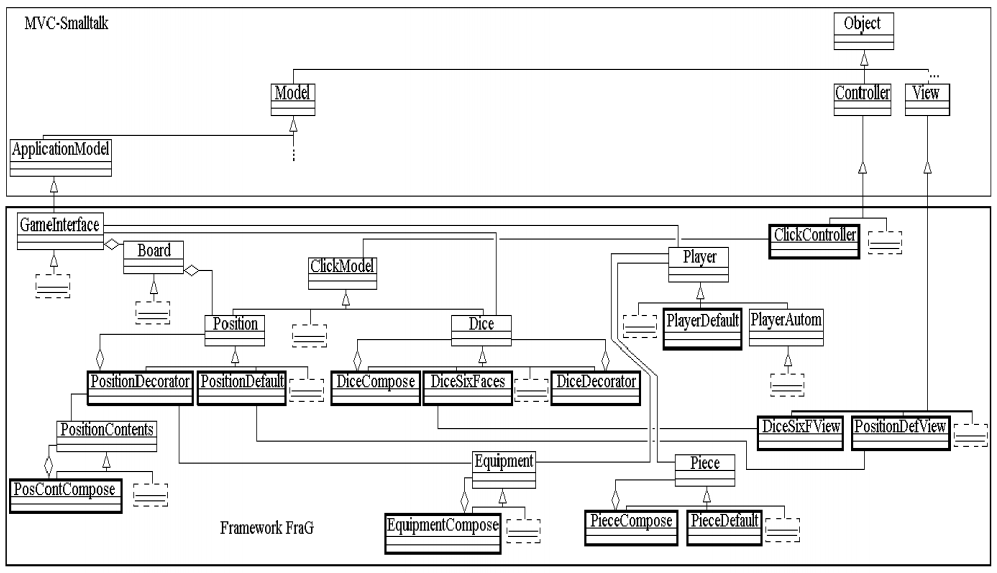
\includegraphics[width=1.0\textwidth]{img/frag.png}
              \end{center}
              \caption{\label{fig:passaro}Modelagem do framework FraG.}
              \begin{center}(FONTE: Adaptado de SILVA, 1998)\end{center}
          \end{figure}

          Dessa forma, o desenvolvedor apenas precisou desenvolver algumas pequenas
          partes para ter uma aplicação totalmente pronta, tendo a maior parte
          do software implementado pelo framework.

          A implementação de um framework consiste principalmente em identificar
          qual domínio de problema ele deve dar suporte. No caso do FraG era um
          framework voltado a desenvolvimento de jogos de tabuleiro. O processo
          de modelagem para um framework requer que o desenvolvedor identifique
          as classes mais comuns de um domínio problema, também conhecidos como
          "hot spots". Esse processo não costuma ser trivial, pois o responsável
          pela modelagem do framework deve estudar ao menos 3 aplicações que compartilham o
          mesmo domínio (JOHNSON, 1993), porém sem se prender muito aos detalhes
          do problema específico.

          Após identificadas as classes que semanticamente são mais utilizadas em um
          certo domínio, inicia-se o processo de modelagem
          que deve definir quais classes deverão ser implementadas e quais serão
          redifinidas pelo desenvolvedor. A partir daí, consegue-se obter resultados
          de quão eficiente o framework desenvolvido é. Para analisar esse dado,
          basta verificar em um projeto que utiliza o framework a porcentagem
          de classes implementadas do zero e quais foram reaproveitadas do framework.
          Isso é claro desconsiderando classes como de interface com o usuário, por
          exemplo, visto que usualmente são totalmente dependendes do domínio da aplicação.

      \section{Aspectos postivos e negativos}
          Quando um framework é utilizado em um projeto de software, é importante estar
          atento aos principais benefícios e problemas em termos de implementação. Quando
          um projeto é feito "from scratch", ou seja, todas as classes são produzidas do
          zero pelo próprio time de desenvolvimento, os programadores tem total liberdade
          para implementar a arquitetura como julgarem melhor. Um exemplo de modelagem desse
          tipo de implementação pode ser melhor observado na Figura 2. Contudo, o problema
          disso, obviamente, é que nada é reusado, a aplicação fica muito suscetível a
          defeitos e demanda muito esforço.

          \begin{figure}[htbp]
              \begin{center}
                  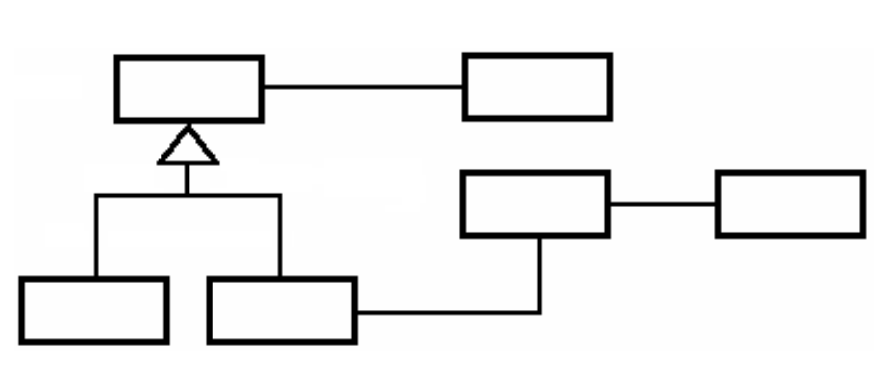
\includegraphics[width=1.0\textwidth]{img/scratch.png}
              \end{center}
              \caption{\label{fig:passaro}Um exemplo de aplicação \textit{from scratch}}
              \begin{center}(FONTE: Adaptado de SILVA, 1998)\end{center}
          \end{figure}

          Quando um framework é utilizado para suprir as necessidades um projeto, muitas
          das classes que inicialmente seriam implementadas do zero, já estão praticamente
          prontas, necessitando, geralmente, apenas de poucas sobrescritas de métodos.
          Os ganhos nesse processo é que os desenvolvedores têm seus esforços
          minimizados, uma vez que boa parte das classes já estão totalmente implementadas.
          Outro aspecto positivo ao se utilizar um framework é que a granularidade do
          reuso é muito maior do que se comparada a um projeto que não usa frameworks.
          Em outras palavras, ao utilizar-se um framework dentro de uma aplicação o reuso
          costuma atingir facilmente dezenas de classes.

          Quanto aos aspectos negativos, o mais fácil de ser observado é que os
          desenvolvedores da aplicação ficam presos à arquitetura e ao controle
          de fluxo de dados impostos pelo framework. Isso ocorre devido ao fato de que, como a
          maioria das classes do domínio do problema já estão sendo implementadas pelo
          framework, tanto a arquitetura como o fluxo de controle já são, por
          definição, pré-estabelecidos.

          Outro grande ponto negativo é que os programadores precisam ter um bom conhecimento
          de como funciona o framework para poder utilizá-lo corretamente. É necessário
          ter conhecimento de como o framework é implementado para saber quais classes
          já foram programadas e acabar não duplicando uma funcionalidade já existente.
          O problema é que para conseguir tais informações os desenvolvedores terão que
          conferir a documentação disponível ou o código fonte. A primeira alternativa,
          apesar de ser a melhor, nem sempre é viável, pois nem sempre é produzida ao
          final de um projeto. Existem casos em que mesmo a documentação não é capaz
          de detalhar o que foi implementado, seja pela não completude ou por não ter
          sido atualizada durante o desenvolvimento do projeto.

          Já a alternativa de analisar o código fonte é, de longe, a maneira mais árdua
          de aprender como a ferramenta funciona. Exige do programador uma atividade
          de engenharia reversa e costuma ter um baixo rendimento. Em alguns cenários
          pode até mesmo deixar o desenvolvedor mais confuso ainda. Isso é claro
          considerando um framework de código aberto, do contrário nem mesmo acesso
          ao fonte o desenvolvedor teria.

      \section{Princípios de frameworks}
          Nessa secção são apresentados alguns conceitos implementados pela maioria
          dos frameworks, mas isso não siginifica que caso algum framework não implemente
          alguma dessas ideias ele não possa ser classificado como tal. Voltando mais uma
          vez ao exemplo do framework do FraG, fica evidente que os frameworks se baseiam
          fortemente nas caracrísticas de associações e heranças.

          É fácil de compreender o motivo pelo qual a herança é tão usada no universo de
          frameworks. Quando utilizada em classes abstratas, por definição, é exigido que
          o programador implemente os métodos abstratos definidos pela superclasse. Isso
          garante que sempre que qualquer objeto que herde a classe abstrata, no momento
          que for utilizado interna ou externamente pelo framework, os métodos estarão
          implementados, o que possibilita uma certa customização dentro do framework e
          é aí que vem a flexibilidade dos frameworks dentro de um domínio de problema.

          Tal fato fica evidente quando observa-se a modelagem do par \textit{Template} e
          \textit{Hook}. Nesse modelo, o método \textit{Template} é um algoritmo sempre
          estável que inicializa objetos que sempre serão necessários para o framework.
          Entretanto, como existem objetos que podem variar de aplicação para aplicação
          ao final da execução do método \textit{Template} o método \textit{Hook} é
          executado. Esse, por sua vez, é um método que deve ser sobrescrito pelo usuário
          para que ele possa inicialzar demais objetos que necessite para sua aplicação.
          Na Figura 3, é possível observar alguns métodos, dentro do framework FraG, que
          são classificados como template ou hook.

          \begin{figure}[htbp]
              \begin{center}
                  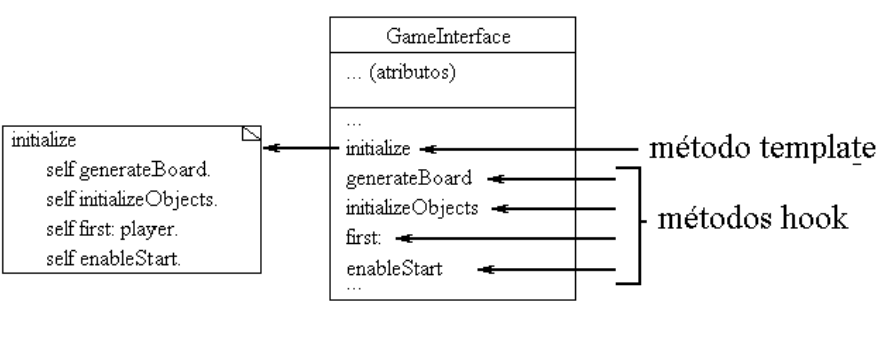
\includegraphics[width=1.0\textwidth]{img/templateHook.png}
              \end{center}
              \caption{\label{fig:passaro}Modelagem dos métodos Template e Hook}
              \begin{center}(FONTE: Adaptado de SILVA, 1998)\end{center}
          \end{figure}

          Outro fato que leva a relação de herança ser tão explorada no mundo de frameworks,
          é o que se chama de princípio de Hollywood (\textit{"Don't call us, we'll call you"}).
          Esse princípio decorre do fato de que quando o desenvolvedor estiver usando a
          ferramenta ele não deve instanciar objetos do framework e chamar métodos. Pelo
          contrário, ele deve criar novas classes que herdem de outras já definidas pelo
          framework. Usualmente, são classes abstratas. Dessa forma, quando a aplicação
          estiver sendo executada, o framework saberá quais classes foram herdadas e
          quais métodos foram escritos. Dessa forma, ele se encarrega de chamar
          os objetos executando corretamente os novos métodos sobrescritos. Daí
          vem o lema: \textit{"Don't call us, we'll call you"}.

          Já o fato de existir tantas relações de associações no framework, vem
          do fato de que os \textit{Design Patterns} são amplamente explorados neste universo de
          soluções. \textit{Design Patterns} são modelagens extremamente
          elegantes e que solucionam problemas que já estão muito bem conhecidos na
          modelagem de software. Na modelagem do FraG, podemos perceber em que há
          casos em que está sendo usado até 3 \textit{Design Patterns} em paralelo:
          \textit{factory, composite, decorator}. Não cabe aqui nesse escopo explanar
          cada um desses \textit{Design Patterns}, muito menos todos os existentes,
          mas é importante deixar claro que cada framework, muito provavelmente, terá
          padrões implementados conforme a necessidade.

          Outro ponto muito forte, é que o framework deve ser capaz de dar suporte a
          uma grande quantidade de aplicações com o mesmo domínio que ele. Como foi
          visto, esse processo na modelagem do framework vem do fato de várias
          aplicações que compartilham o mesmo domínio terem sido exaustivamente
          estudas e terem seus módulos semelhantes identificados e implementados
          de forma genérica na nova ferramenta. Feita essa parte, basta que
          os desenvolvedores escolham precisamente quais classes devem ser reescritas
          em cada projeto, e terão boa parte da implementação já realizada e testada.

  % ---
  \chapter{Testes}
  % ---
      Nos primórdios da história do desenvolvimento de software, a etapa de testes
      era geralmente um parte vista com maus olhos pelos programadores e rotineiramente
      só se realizava quando "sobrava tempo" no projeto. Com o passar do tempo, foi
      ficando evidente para as empresas que a parte de testes é essencial para
      assegurar a qualidade do produto (WAZLAWICK, 2012). Ela não só é importante
      para comprovar o correto funcionamento, como também ajuda a garantir
      estabilidade durante a refatoração de código, pois se um teste estava obtendo
      sucesso antes da alteração e passou apresentar falhas depois das mudanças é
      porque certamente houve algum equívoco por parte de quem alterou o código.

      Nessa parte do trabalho é de suma importância deixar esclarecido
      que um projeto que foi conduzido sem testes, pode atigingir um patamar
      satifatório de qualidade ao longo do processo, mas isso provavelmente terá um
      custo alto, em que o programador segue a filosofia do \textit{code and fix},
      em que a medida que ele vai codificando, vai arrumando os erros que encontra.
      Sendo assim, o time de desenvolvimento terá que gastar mais tempo arrumando
      falhas que poderiam ter sido percebidas mais cedo. Isso faz com que o tempo
      de projeto aumente bem como os custos. Dessa forma é sempre importante que
      a parte de testes esteja prevista no planejamento inicial de um projeto de software.

      É importante deixar claro, desde já, que o teste de software em momento
      algum supõe que o módulo implementado esteja livre de defeitos. A única coisa que o
      teste garante para o desenvolvedor é que para as entradas especificadas o
      componente está se comportando como o programador desejava. O teste costuma
      ser implementado pensando em como fazer com que o módulo dê problemas, mas
      também não esquecendo da \textit{happy path}, também conhecido como sequência
      de estados em que não há ações inválidas. O teste é, então, nada mais que um conjunto
      de código que coloca o módulo que está sendo testado em um determinado estado,
      ou seja com valores específicos para as variáveis e analisa como o módulo está
      reagindo.

      Pensando em um cenário mais prático, propõe-se um módulo simples em que a única
      responsabilidade é verificar se um dado CPF é válido ou não, mesmo que possua uma
      máscara. Abaixo, podem-se observar, na Figura 4, as assinaturas de método do
      mesmo na linguagem
      \textit{Python}.

      \begin{figure}[htpb]
          \begin{lstlisting}
              class CpfValidator(object):
                def __init__(self):
                  # TODO
                  pass

                def cpf_is_valid(cpf):
                  # TODO
                  pass

                def cpf_with_mask_is_valid(cpf_with_mask):
                  # TODO
                  pass
          \end{lstlisting}
          \caption{\label{fig:passaro}Módulo com assinaturas de método para validar CPF}\vspace{-1.2\baselineskip}
          \centering
          \begin{center}(FONTE: Imagem feita pelo autor)\end{center}
      \end{figure}

      Apesar de nenhum dos métodos ter sido realmente implementado, é perfeitamente
      possível desenvolver um arquivo de teste para esse módulo. Basta que o programador
      tenha conhecimento do algoritmo de validação de CPF. Dessa forma, ele saberá quando
      um CPF é válido mesmo estando sem a máscara (i.e. formatação). Ou seja, quando
      o teste for implementado basta ele escrever que os CPFs que obedeçam o algoritmo
      devam ser classificados como válidos, enquanto que os inválidos devem ser
      rejeitados. Com o teste desenvolvido, basta o programador executá-lo e
      obviamente o teste retornará uma mensagem de erro, isso porque o módulo ainda não
      foi implementado. Caso o teste retorne somente mensagens de sucesso é porque o
      teste possui algum equívoco.

      Com o teste produzido, o progamador dever seguir aquilo que é conhecido como
      \textit{baby steps}. O teste, uma vez escrito e executado, dirá qual o erro
      que está acontecendo, seja função não implementada, método retornando valores
      incorretos, objeto nulo. Dessa forma, o desenvolvedor irá corrigir o erro e
      irá executar novamente. Provalvelmente na segunda iteração, o teste apontará
      um novo erro. O programador deve, então, proseguir nesse processo até que o
      teste retorne somente mensagens de sucesso.

      Esse processo é também conhecido como desenvolvimento orientado a testes, cuja
      a sigla em inglês é TDD. A Figura 5 seguinte ilustra bem esse processo e que
      também é conhecido como \textit{red, green and refactor}, já que o programdor
      começa inicialmente na fase de erros (\textit{red}), faz somente o necessário
      para que o módulo passe no teste (\textit{green}) e melhora no final a qualidade
      do código a medida do necessário (\textit{refactor}) (BECK, 2004).

      \begin{figure}[htbp]
          \begin{center}
              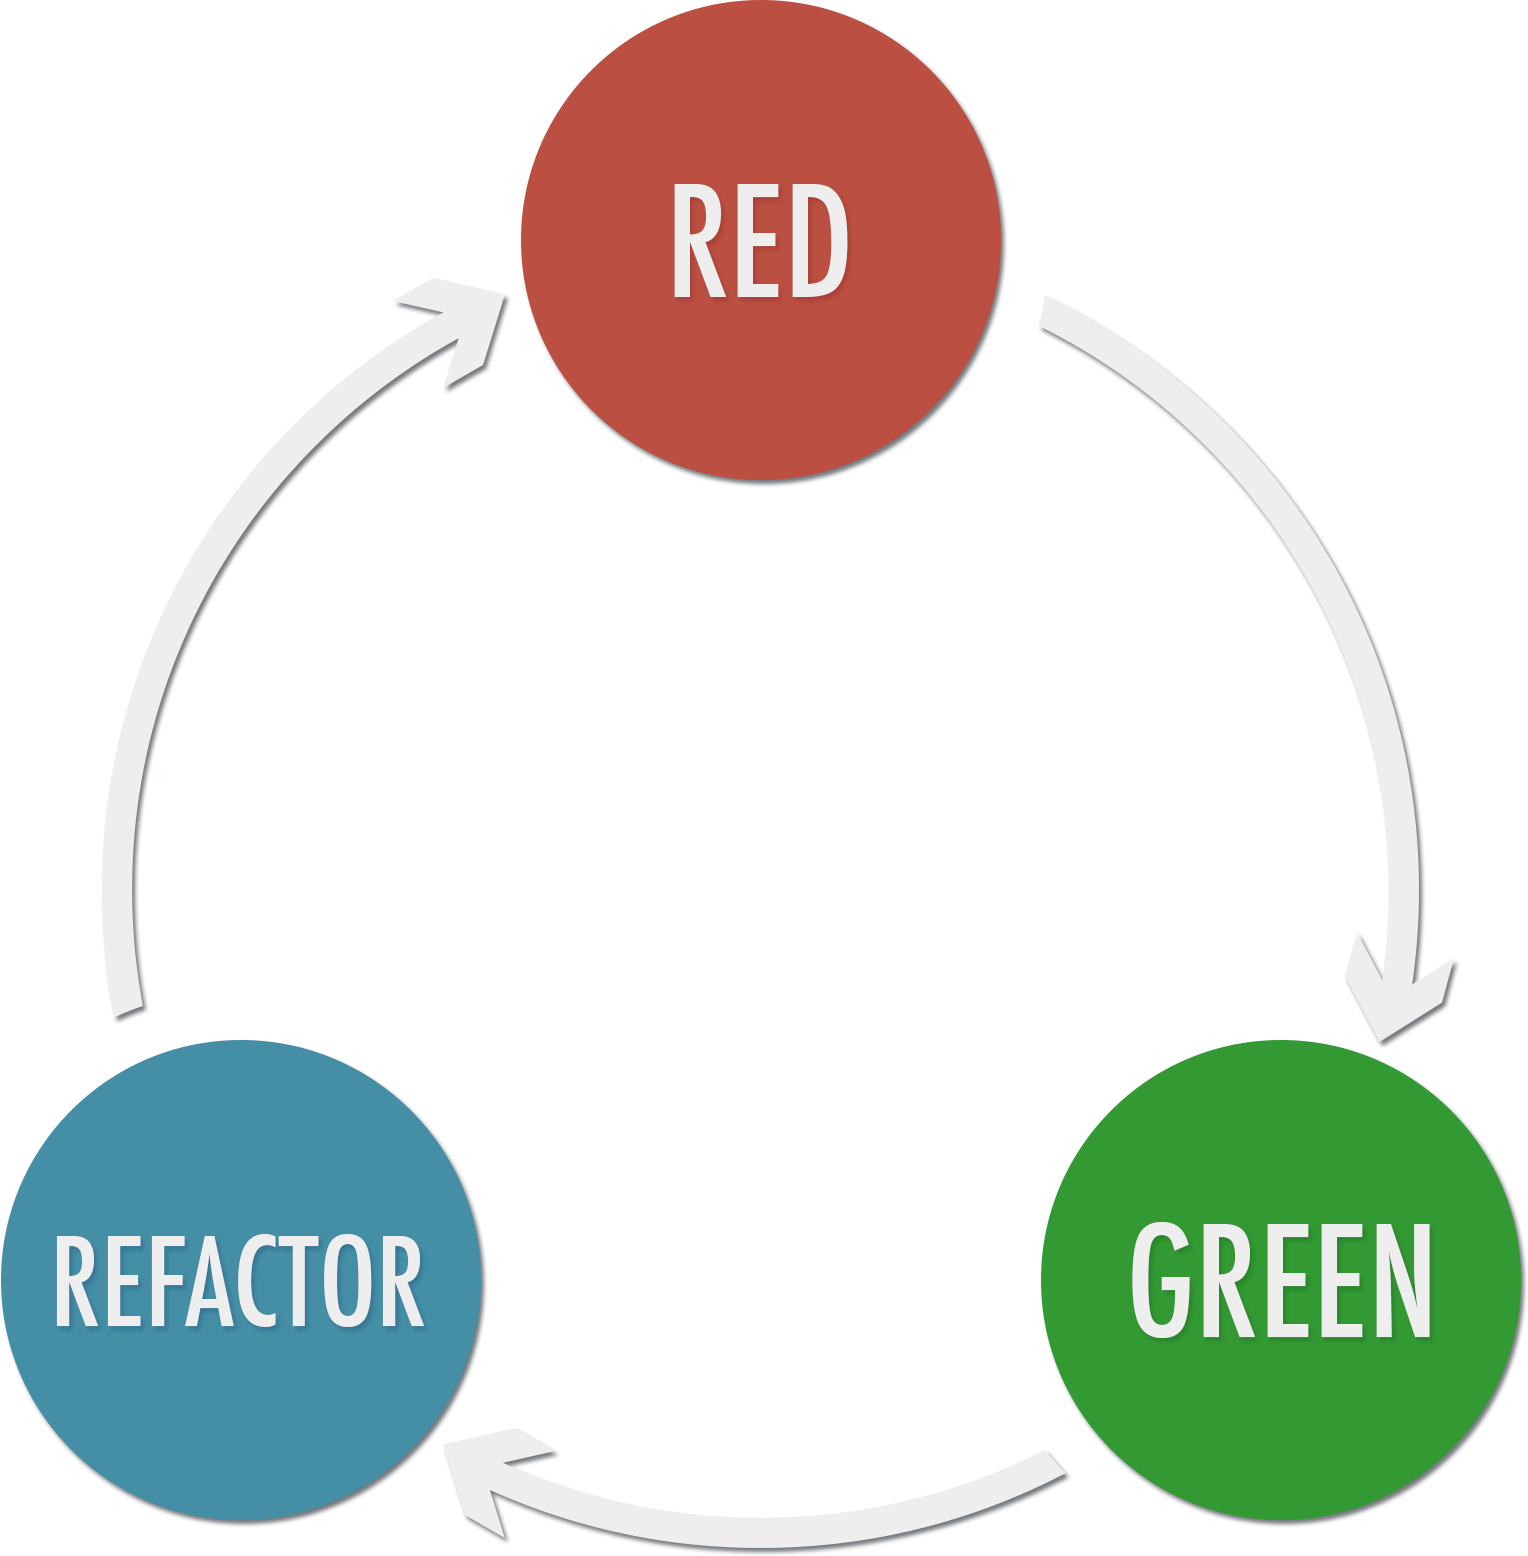
\includegraphics[width=0.4\textwidth]{img/rgf.png}
          \end{center}
          \caption{\label{fig:passaro}Diagrama que representa o padrão RGF}
          \begin{center}(FONTE: Adaptado de FOWLER, 2014)\end{center}
      \end{figure}

      Ainda no contexto de desenvolvimento de testes, é importante que os desenvolvedores
      e o time de qualidade estejam constantemente refatorando o código produzido por
      cada um. Isso é importante, pois quem está desenvolvendo o módulo já sabe como
      o código funciona e fica mais difícil em perceber o local do defeito. Entretanto,
      quando alguém que não desenvolveu o componente começa a se familarizar mais com o código
      ela vai, usualmente, ler cada linha do código e tentar enteder a semântica de cada
      uma delas. Dessa forma, ficará muito mais evidente para quem está de fora identificar
      o erro. Por isso, os cenários de teste devem ser sempre atualizados e refatorados
      (REID, 2016).

      Outro ponto importante a ser ressaltado é a questão das \textit{pré e pós condições} de
      um dado caso de teste. A pré-condição é uma obrigatoriedade que deve ocorrer
      antes que um dado método inicialize. Pensando num exemplo mais prático,
      imagina-se uma outra classe que executa algum procedimento depois de a classe
      de validaçao de CPF ter comprovado que o dado informado está correto. Nos métodos
      que essa nova classe implementa, o desenvolvedor não precisa se preocupar se o
      dado está correto ou não, pois a classe anterior já o fez. Isso é o que se chama
      de pré-condição. Já a pós-condição é o estado que o sistema deve se encontrar
      após o procedimento ter sido executado. Muitas vezes, o teste deve verificar
      se o sistema chegou no estado esperado. No mesmo exemplo, supõe-se que a nova
      classe pesquise no banco o usuário pelo CPF e mande um email para o mesmo. Para
      ver se a pós-condição foi atendida, o sistema deve verificar se o servidor de
      emails mandou um email para o usuário com aquele CPF.

      Nos dias atuais, o mercado é repleto de ferramentas e frameworks capazes de
      auxiliar os desenvolvedores durante a implementação de testes, fornecendo
      objetos falsos, também conhecidos como \textit{mocks}, funções de asserção,
      execução de testes em ordem aleatória. Como o intuito de trabalho é desenvolver
      um framework que seja capaz de automatizar a produção de testes, esse capítulo
      tratará essencialmente de tipos de teste, níveis e técnicas de teste. Neste trabalho,
      testes relacionados a segurança e desempenho, como de carga e stress, não serão
      contemplados, pois fogem do escopo do que o trabalho se propõe a fazer.

      \section{Modelagem e implementação de testes}
          A modelagem de testes é uma fase importante, visto que é responsável
          por garantir o mínimo de qualidade no módulo que está sendo implementado.
          O desenvolvimento de uma aplicação pode seguir a filosofia TDD em que o
          programador primeiro implementa o teste e depois desenvolva o módulo que
          lhe foi designado. Porém, nada impede que o desenvolvedor implemente
          inicialmente o módulo e depois avançe para a parte de teste.

          Entretanto, durante a modelagem de testes, o mínimo que o desenvolvedor precisa
          conhecer para poder implementar o teste são os métodos do artefeato que
          lhe foi atribuido, bem como a ideia de seus algoritmos. Dessa forma ele
          consegue separar as entradas para o teste em dois grandes conjuntos: o
          conjunto das entradas válidas e das inválidas. De posse de tais informações
          básicas, ele pode escrever testes que seguem o \textit{happy path} e aqueles
          que devem lançar algum tipo de exceção.

          Para deixar mais claro, retorna-se ao exemplo do módulo de validação de CPF
          escrito em \textit{Python}. Como pode-se perceber pelo código fornecido na
          Figura 4, é facilmente perceptível que a linguagem é \textbf{fracamente tipada},
          ou seja, é deixado ao interpretador inferir a tipagem de cada variável. Para
          efeitos práticos, será considerado que os parâmetros fornecidos para os dois
          métodos de validação sejam do tipo \textit{string}. Um possível cenário de teste
          que segue o \textit{happy path} seria fornecer um CPF válido e o teste iria
          retornar dizendo que tudo ocorreu como esperado. Por outro lado, se em algum
          cenário de teste em que seja fornecida uma sequência de inteiros, o correto
          seria que o módulo lançasse alguma exeção do tipo \textit{InvalidType} e o
          teste detectasse que essa exeção foi lançada. Ao perceber que houve uma exceção
          o teste deve informar, novamente, tudo ocorreu como esperado. Do contrário, ele
          deve trazer um relatório escrito dizendo que estava sendo esperado uma exceção,
          porém a mesma não ocorreu.

          Na modelagem de testes é importante também que durante a implementação exista
          o teste de entradas aleatórias para simular uma possível simulação com o usuário.
          Nos dias atuais, existem várias bibliotecas capazes de gerar dados falsos que
          cumprem com este objetivo e são capazes de criar informações falsas, porém válidas,
          como: nomes, emails, senhas, cartões de crédito, CPF. Sendo assim, é importante
          também que durante a modelagem de teste o desenvolvedor preveja ao menos um cenário
          em que ele possa tirar proveito dessas bibliotecas.

          A modelagem de teste em si pode ser abordada de inúmeras formas. Dentro da ciência
          da computação, o mais comum é enxergar o teste do módulo como sendo um \textbf{
          autômato finito}. Os estados representam o objeto em si e as transições
          seriam os métodos e os possíveis valores de retorno, ou execções, dependendo dos
          valores passados para o método. O objetivo do teste, vendo a modelagem por essa
          ótica, seria  verificar se a máquina chegou num estado de aceitação, ou não.
          Nesse sentido, é possível ver o autômato representando o teste para a validação de
          um CPF, do módulo representado anteriormente, na Figura 6.

          \begin{figure}[!htb]
              \begin{center}
                  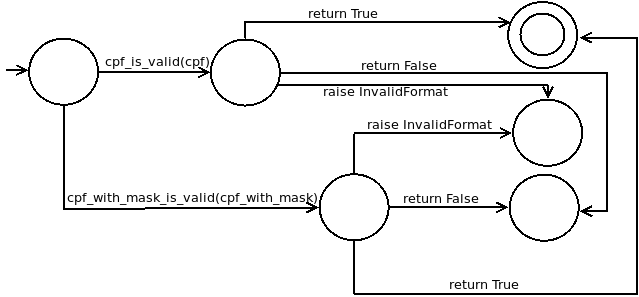
\includegraphics[width=0.80\textwidth]{img/afd.png}
              \end{center}
              \caption{\label{fig:passaro}Diagrama que representa o teste do módulo de CPF na ótica de AFD}
              \begin{center}(FONTE: Imagem feita pelo autor)\end{center}
          \end{figure}

          Olhando para o autômato descrito, o desenvolvedor se quisesse garantir
          o máximo de qualidade possível, teria que testar todos os caminhos possíveis
          partindo do estado inicial. Nesse exemplo, a tarefa de testar o módulo é perfeitamente
          realizável, uma vez que existem poucas transições. Porém, pensando em casos mais
          reais em que os módulos possuem pelo menos de 6 a 8 procedimentos e que podem ter
          suas próprias execeções, a tarefa de testar completamente um artefato começa a ficar
          inviável. Nesse sentido, o programador deve priorizar as entradas mais comuns
          e algumas exóticas para garantir uma certa qualidade.

          Ainda dentro do contexto do autômato, é importante lembrar que não foram representadas
          mais transições dos estados mais à direita em direção a outros estados por uma mera
          questão de legibilidade. Entretanto, dentro de um contexto de um objeto que é utilizado
          várias vezes, a chamada repetitiva de vários métodos sucessivamente pode acarretar,
          eventualmente, na mudança de algum atributo que poderia encadear alguma mudança no
          comportamente do método, dependendo do algoritmo implementado. Sendo assim, é importante
          que o programador tenha em mente essas possibilidades também.

          Já no que se refere à parte de implementação, a implementação do padrão de projeto
          \textit{factory} (FOWLER, 2003) costuma ser muito comum, visto que é uma solução elegante
          para os testes. Esse padrão se faz essencial para manter um código mais limpo,
          visto que em cada cenário de teste o desenvolvedor precisará de objetos com valores de
          atributos diferentes. Dessa forma, ele pode usar uma biblioteca que implemente a
          o padrão para os objetos necessários para o teste e para cada cenário ele solicita
          objetos diferentes para a fábrica. Isso ajuda a manter um código mais legível, visto
          que se esse padrão não fosse utilizado, para cada teste o programador teria que sempre
          estar instanciando um objeto da mesma classe e configurando os valores manualmente,
          o que, por sua vez, não segue o príncipio básico do DRY (\textit{Don't repeat youself}).

      \section{Níveis de teste}
          Dentro do universo de teste de software, pode-se classificar os testes pelos seus
          níveis ou fases. A classificação decorre do fato de que a medida que a aplicação
          vai crescendo os testes também precisam ter uma complexidade maior, pois o número
          de combinações de entradas possíveis do usuário vai aumentando. Classicamente,
          (WAZLAWICK, 2012), os testes, quando dividos dessa forma, podem pertencer alguma
          dessas classes: unidade, integração, sistema, aceitação e o de regressão. O
          conceito de níveis deriva daquilo que é conhecido por \textit{Pirâmide de testes},
          ilustrada na Figura 7. A pirâmide de testes correlaciona a quandidade de cada nível
          de teste junto com seus custos e tempo de execução. Na base da pirâmide, portanto,
          identifica-se os testes com maior expressividade, em número, e que exigem pouco
          esforço para serem programados e que executam mais rapidamente, enquanto que no topo
          é justamente o inverso. Nas próximas subsecções serão apresentados brevemente cada
          uma dessas classificações de níveis.

          \begin{figure}[!htb]
              \begin{center}
                  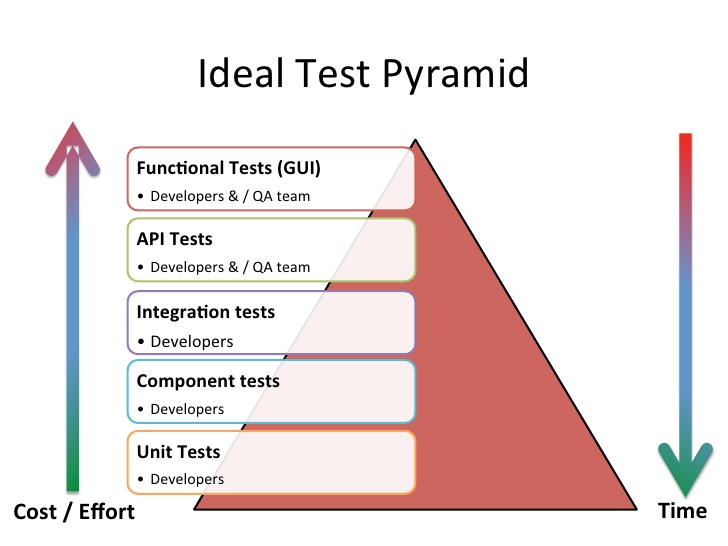
\includegraphics[width=0.55\textwidth]{img/pyramid.jpg}
              \end{center}
              \caption{\label{fig:passaro}Pirâmide que correlaciona quantidade de cada nível de teste}
              \begin{center}(FONTE: Adaptado de BAGMAR, 2012)\end{center}
          \end{figure}

          \subsection{Teste de unidade}
              O teste de unidade é o teste mais básico de um software. O intuito dele é basicamente
              testar a classe que está para ser implementada ou que recém foi programada. Boa
              parte dos testes de uma aplicação são classificados dessa forma, uma vez que são
              os mais baratos de serem desenvolvidos e os mais rápidos de serem executados (FOWLER, 2012).
              Este nível de teste visa somente fazer o teste de uma classe isolada. Caso a classe
              que está sendo testada iteraja de alguma forma com outras classes, seja por atributos
              ou parâmetros de métodos, o programador, deve, então, usar objetos falsos, também
              conhecidos como \textit{mocks}, para simular a classe que possui relação com a classe
              que está sendo testada. Essa metodologia garante que caso qualquer defeito detectado
              pelo teste, o defeito vem unica e exclusivamente da classe que está sendo testada,
              e não de classes terceiras.

          \subsection{Teste de integração}
              Como o nome já sugere, o objetivo desse teste é garantir a qualidade de dois ou mais
              módulos que trabalham em conjunto. Nesse nível deve-se testar todos os módulos que possuêm
              alguma relação do tipo: associação, composição ou agregação. Ao invés de usar objetos
              falsos, como era feito no nível anterior, usam-se objetos verdadeiros e testam-se os
              métodos pelos quais estes objetos trocam mensagens. Em casos em que um dos módulos
              estava funcionando no teste de unidade e passou a não funcionar no teste de integração,
              é porque muito provalmente o módulo que foi integrado está com algum problema. Este tipo
              de teste não deve cobrir integrações com com sistemas de terceiros, APIs por exemplo.

          \subsection{Teste de sistema}
              O teste de sistema é o teste em que os desenvolvedores utilizam o sistema no modo de
              produção fingindo ser um usuário comum e simulando suas respectivas ações. Esse teste,
              geralmente usa como base algum caso de uso descrito no processo de engenharia de
              requisitos e também busca achar eventuais defeitos na interface de usuário. Esse
              teste atualmente pode ser facilmente automatizado, mas como a interface é um componente
              que usulamente está sendo alterada, algumas empresas ainda preferem realizá-lo de maneira
              manual e automatizar somente quando a interface já está bem estabelecida.

          \subsection{Teste de aceitação}
              O teste aceitação é o teste mais importante de todos, pois é nesse teste em que o
              usuário utiliza o sistema sem auxílio dos desenvolvedores. Ele é o mais importante,
              pois o cliente dirá se as funcionalidades requisitadas foram cumpridas e valida
              se a coleta de requisitos foi feito da forma correta.

          \subsection{Teste de regressão}
              O teste de regressão é um nível de teste que busca executar toda a base de
              testes para um sistema que foi recém refatorado ou que teve uma nova versão lançada.
              O nome vem do fato de que caso o sistema que foi atualizado estava sendo aprovado
              nos testes e passou a ter erros, é dito, então, que o sistema regrediu (WAZLAWICK, 2012).

      \section{Técnicas de teste}
          As técnicas de teste indicam a forma como os casos de teste serão implementados.
          Todas elas possuem em comum encontrar falhas no artefato desenvolvido. As principais
          técnicas que podem ser aplicadas são: caixa-branca, caixa-preta e caixa-cinza. Os próximos
          tópicos detalharão cada uma dessas técnicas.

          \subsection{Técnica da caixa preta}
              É também conhecida como teste comportamental e, usualmente, é a técnica mais aplicada.
              O desenvolvedor fornece um conjunto de entradas e utiliza uma função de asserção
              para avaliar o resultado retornado, sem se preocupar com a execução interna do código.
              Essa técnica pode ser aplicada em qualquer nível de teste. Obviamente, quanto mais
              entradas sejam testadas, melhor o teste é. Como já foi dito anteriormente, é
              impossível testar todas as entradas possíveis. Nesse caso, o programador pode utilizar
              classes de equivalência para maximizar os casos de teste coberto. As classes de equivalência
              nada mais são do que dois subconjuntos do universo do conjunto de entradas possíveis,
              em que um subconjunto representa as entradas válidas e o outro as entradas inválidas.
              Uma abstração dessa técnica pode ser contemplada na Figura 8.

              \begin{figure}[htbp]
                  \begin{center}
                      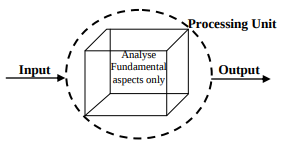
\includegraphics[width=0.7\textwidth]{img/blackbox.png}
                  \end{center}
              \caption{\label{fig:passaro}Visão da técnica da caixa preta}
              \begin{center}(FONTE: Adaptado de KHAN, 2012)\end{center}
              \end{figure}

              A filosofia por trás dessa técnica, encontra-se na ideia de que basta o programador
              saber o que um determinado método deveria retornar para um certo parâmetro
              \textit{X}. Para melhor exemplificar essa ideia, propõe-se mais adiante um módulo
              escrito na linguagem \textit{Python} capaz de fazer cálculo da função fatorial.
              O módulo pode ser observado na Figura 9. Mesmo que, por um
              acaso, o progamador não soubesse como a função fatorial funcionasse ou se ainda ela
              fosse muito complexa envolvendo cálculos matemáticos avançados, basta que ele saiba que
              fornecendo um valor \textit{X}, o método deve retornar obrigatoriamente
              \textit{X*(X-1)*(X-2)*...*1}.

              Dessa forma, ao criar um teste para esse método basta que o programador escreva que
              quando o algoritmo for executado com o valor 4, por exemplo, deve ser retornado
              o valor 24. Caso seja retornado qualquer coisa diferente desse valor ou uma mensagem
              de erro é porque, então, existe um defeito no módulo implementado. É claro que a
              a função de cálculo de fatorial é um algoritmo trivial de ser testado. Porém, em
              projetos mais complexos de software há a necessidade de se explicitar o que cada
              método deve retornar a fim de que quem escrever um teste baseado na técnica da caixa
              preta possa fazê-lo sem saber como o método é realmente implementado.

              \begin{figure}[!htbp]
                  \begin{lstlisting}
                      class FactorialCalculator(object):
                        def __init__(self):
                          pass

                        def factorial(n):
                          result = 1
                          while (n != 0):
                            result *= n
                            n -= 1
                          return result

                  \end{lstlisting}
                  \caption{\label{fig:passaro}Módulo com implementação de método que calcula fatorial}
                  \begin{center}(FONTE: Imagem feita pelo autor)\end{center}
              \end{figure}

              Usualmente, nesse tipo de técnica, costuma-se buscar valores limites para verificar
              se o módulo está se comportando como deveria, uma vez que os defeitos de um software
              costumam ficar em suas frestas (WAZLAWICK, 2012). Considerando que o método recebe somente
              valores inteiros, o algoritmo possui uma grande falha no que se refere as frestas. Ele,
              apesar de calcular corretamente os valores para qualquer inteiro não negativo, se
              eventualmente o método for executado usando como parâmetro um inteiro negativo, então o
              módulo ficará computando eternamente.

              Aplicando o princípio dos conjuntos de equivalência para um possível arquivo de teste
              para este módulo, o desenvolvedor poderia criar testes usando os seguintes valores como
              parâmetro: -2, -1, 0, 1 e 2. Para os valores negativos, o programa, necessariamente deveria
              lançar uma exceção e o teste, ao receber a exceção, deveria afirmar que tudo ocorreu como
              esperado. Nesse caso, para arrumar o módulo implementado, ao em vez de usar o
              operador de diferença, basta utilizar o operador de >. Para os demais valores, basta criar
              os casos de teste utilizando a técnica da caixa preta como foi descrita anteriormente.

          \subsection{Técnica da caixa branca}
              A técnica da caixa branca, por sua vez, é uma técnica muito mais robusta que se comparada
              a da caixa preta. A ideia consiste em testar qual fluxo o código está sendo executado no
              componente. Esse tipo de teste visa, além de busca de erros, eliminiar trechos que nunca
              são alcançados dentro de um método ou que sejam reduntantes. Quando esta técnica é
              aplicada todas as possibilidades de fluxo de um método devem ser testados
              (i.e. \textit{while, for, if, else, try, catch, finally}).

              Esse tipo de teste não necessariamente procura erros dentro de um módulo, mas busca
              otimizá-lo, em termos de processamento. Isso decorre do fato de que, podem haver
              estruturas de controle de fluxo que estão sendo declaradas, mas nunca são alcançadas.
              Ou seja, o módulo está funcionando corretamente, justamente por tais estruturas não
              estarem sendo executas. Dessa forma, a finalidade do teste é diminuir as linhas de código
              e deixar ele com um desempenho ainda maior.

              Nessa subsecção, cabe um comentário para complementar o que foi apresentado quanto a
              questão de modelagem de testes baseado em autômatos. Conforme Wazlawick (2012 em p. 400) é
              apresentada uma forma de modelar testes, baseados nessa técnica. A ideia consiste em
              modelar um autômato finito em que que cada nodo representa uma linha ou um conjunto de
              linhas sequenciais que contenham no máximo uma estrutura de controle e as arestas
              representam o atendimento ou não da condição imposta pela estrutura. A modelagem
              com esse tipo autômato para o método de cálculo de fatorial pode ser visto na Figura 10.

              Através do diagrama, é percebido que, então, o princípio do teste é passar por todas as
              arestas do automâto e caso alguma aresta em nenhuma hipótese seja utilizada é porque a
              estrutura jamais é alcançada ou possui uma condição impossível de ser atendida.

              \begin{figure}[htbp]
                  \begin{center}
                      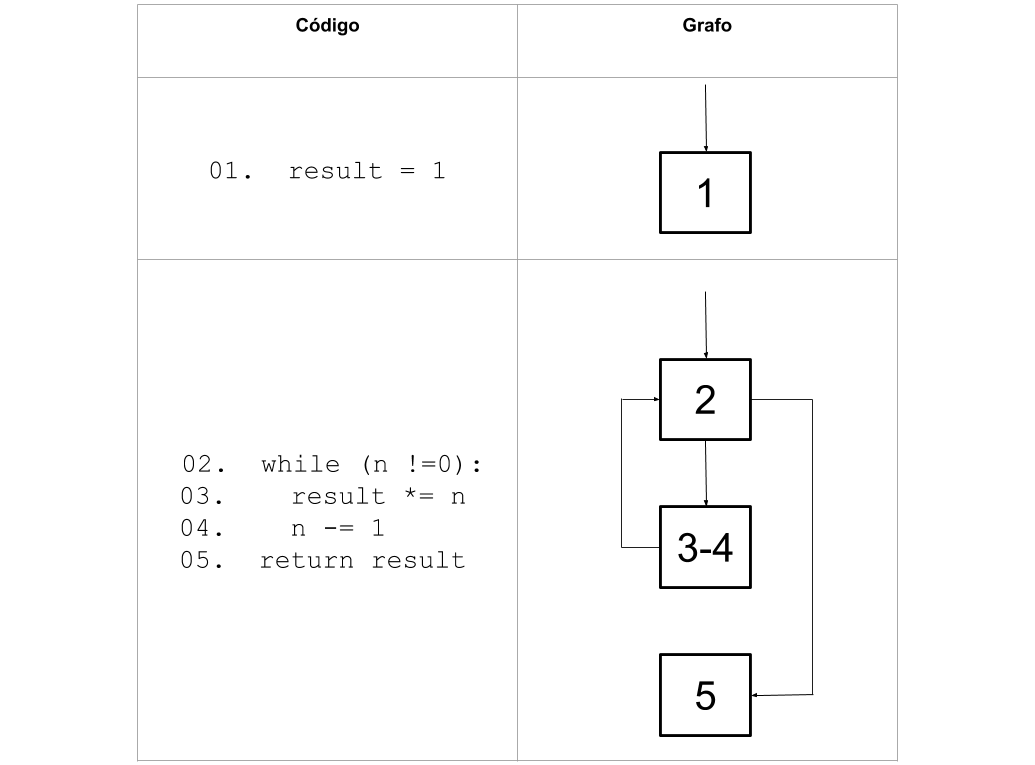
\includegraphics[width=1.0\textwidth]{img/whitebox.png}
                  \end{center}
              \caption{\label{fig:passaro}Visão da técnica da caixa branca usando AFD.}
              \begin{center}(FONTE: Imagem feita pelo autor)\end{center}
              \end{figure}

              Fica evidente pela figura que quanto mais arestas o autômato possui (i.e. estruturas
              condicionais), fica mais complexo de se testar o módulo. Isso mostra a importância clara de
              que todo método deve ter no máximo 20 linhas, pois além de ser mais trivial de ser testado,
              mantém uma maior legibilidade.

          \subsection{Técnica da caixa cinza}
              Essa técnica tem por finalidade combinar as duas técnicas apresentadas anteriormente em uma
              só. A caixa cinza baseia-se em testar quais são as saídas para cada uma das entradas
              fornecidas, bem como rastrear quais foram os trechos que foram executados para gerar aquele
              resultado e avaliar se faz sentido, ou não. Utilizando o exemplo do fatorial, imaginando
              um cenário que o desenvolvedor fornece como parâmetro o valor 4 ele deveria obrigatoriamente
              retornar o valor 24. Mas, mais do que isso, a estrutura de controle \textit{while} deveria
              ser executada 4 vezes e depois retornar o valor esperado.

  % ---
  \chapter{Desenvolvimento Mobile}
  % ---

      O desenvolvimento de aplicações mobile, foi uma área que existiu desde o início dos
      primeiros dispositivos móveis, mas que ganhou mais destaque nos últimos anos, como visto na
      Figura 11. Nas primeiras gerações de celulares com interface gráficas e com capacidade
      de processamento mais robusta, uma séries de aplicativos era disponibilizada ao usuário como:
      agenda, calendário, email, jogos e até mesmo acesso a internet. Porém, por mais variadas que as
      aplicações fossem, o usuário não podia instalar aplicativos de terceiros, pelo menos não de uma
      maneira que fosse simples para um usuário leigo. Geralmente o processo envolvia baixar
      conteúdo de desenvolvedores no computador e fazer o deploy manualmente.

      \begin{figure}[htbp]
            \begin{center}
                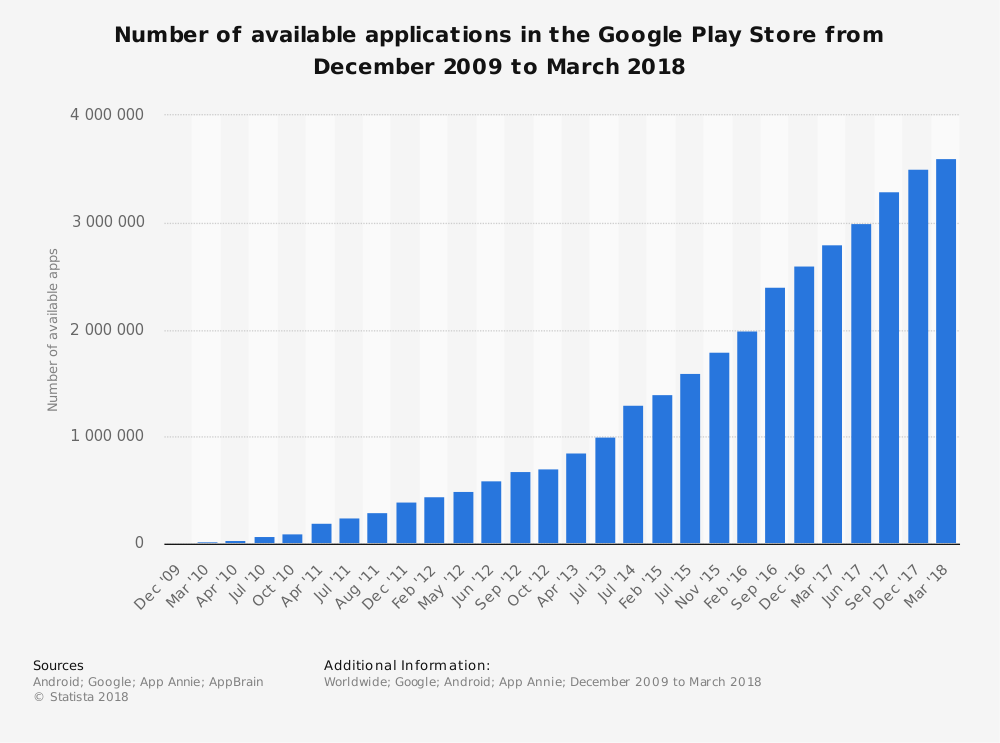
\includegraphics[width=0.65\textwidth]{img/numberApps.png}
            \end{center}
        \caption{\label{fig:passaro}Número de aplicações disponível na Google Play ao passar dos anos}
        \begin{center}(FONTE: Statista, 2018)\end{center}
      \end{figure}

      Com o passar dos anos, a indústria de dispositivos mobile passou por um processo muito
      semelhante ao que houve no mundo de computadores desktop, tanto no quesito hardware quanto
      software. Os componentes eletrônicos para essas plataformas foram ficando cada vez mais
      poderosos e baratos ao longo dos anos (HALPERN, 2016). Já no que se refere aos sistemas
      operacionais, o mercado, aos poucos, foi convergindo para um número menor de sistemas. Dessa
      forma, surgiram sistemas operacionais que hoje, praticamente, dominam totalmente o mercado de
      dispositivos móveis, como pode ser observado na Figura 12. São esses: Android, iOS e
      Microsoft Phone, produzidos respectivamente pela Google, Apple e Microsoft.

      Com um mercado renovado, os desenvolvedores passaram a ter uma maior liberdade para poder
      desenvolver suas aplicações. Porém, o que fez com que esse mercado ficasse tão em voga
      como está nos dias de hoje foi o fato de que as empresas responsáveis pelos sistemas
      operacionais disponibilzassem aos seus usuários uma loja virtual de aplicativos.
      Isso fez com que os usuários não ficassem mais limitados única e exclusivamente
      às aplicações que viam de fábrica. Outro fator que fez com que o mercado criasse
      essa grande necessidade por aplicações mobile foi a facilidade que muitas das
      empresas dão aos desenvolvedores em disponibilizar seus aplicativos nessas mesmas
      lojas, fosse de forma gratuita ou não.

      Porém, semelhante aos softwares para as plataformas desktop, o desenvolvimento de aplicações
      mobile não é absultamente perfeito. O maior problema para desenvolvedores que almejam
      ter suas aplicações disponíveis em todas as plataformas, é o da linguagem de programação.
      Enquanto que o ambiente da Google suporta apenas Java e Kotlin, o iOS era uma plataforma
      que exigia que os programadores programassem em Objective-C, mas que agora usa como linguagem
      nativa o Swift. Por último, a Microsoft possui como linguagem padrão o Visual C++ e o C\#.
      Dessa forma, por mais que uma aplicação mobile seja bem projetada, do ponto de vista de
      orientação a objetos, sempre será necessário replicar a aplicação para outra linguagem,
      seja através de um transpilador ou de trabalho puramente manual. Por tal razão, o foco
      desse trabalho focará exclusivamente na plataforma Android.

      \begin{figure}[htbp]
            \begin{center}
                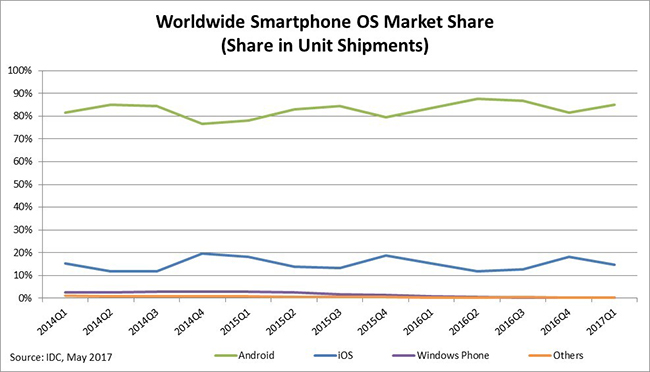
\includegraphics[width=0.7\textwidth]{img/osPercentage.jpg}
            \end{center}
        \caption{\label{fig:passaro}Porcentagem de sistema operacional por dispositivo móvel}
        \begin{center}(FONTE: IDC, 2017)\end{center}
      \end{figure}

      Nesse sentido, nas próximas secções será apresentado uma breve abordagem técnica do
      Android, seguido de uma secção que tratará do desenvolvimento de aplicações nessa
      mesma plataforma, trazendo os principais aspectos e conceitos

      \section{Especificações técnicas do Android}
        O Android foi uma plataforma que teve seu primeiro lançamento, oficial, em 2008. Na época,
        a divisão que desenvolveu o sistema já pertencia a Google. O objetivo inicial do projeto,
        era desenvolver um sistema operacional para celulares capaz de identificar a localização
        do usuário e suas principais preferências. No que se refere a termos de licença, o Android
        possui uma licença própria criada pela Google conhecida como AOSP (Android Open Source
        Project), ou seja uma licença de código aberto.

        O Android, atualmente, é baseado em uma das versões do kernel do Linux, mais especificamente
        as versões: 3.18 e 4.4, dependendo do aparelho. Apesar de o Android ter o kernel baseado
        em versões LTS (Long Term Support), muitas modificações tiveram que ser feitas para atender
        aos requisitos da Google. Uma das principais mudanças foi que a Google teve que desenvolver
        uma biblioteca alternativa a GNU C, visto que os processadores que iriam executar o sistema
        eram CPU's com baixa frequências. A biblioteca ficou conhecida como \textit{Bionic}.

        As principais arquiteturas suportadas atualmente pelo Android são a ARM, x86 e MIPS. Como
        pode ser visto no gráfico seguinte, a arquitetura ARM é a dominante, visto que é uma ISA
        (Instruction Set Architecture) que preza pela eficiência energética. Já quanto ao x86 e
        o MIPS foram arquiteturas que foram ganhar suporte somente mais tarde, visto que essas eram
        as arquiteturas utilizadas nos computadores dos desenvolvedores que emulavam as aplicações
        Android. Mais recentemetne, as versões 64 bits dessas mesmas ISA estão, gradativamente,
        ganhando suporte da plataforma.

        \begin{figure}[htbp]
            \begin{center}
                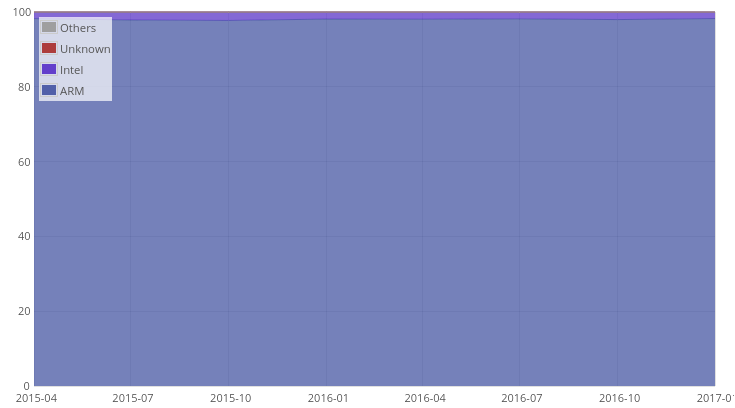
\includegraphics[width=0.7\textwidth]{img/cpusPercentage.png}
            \end{center}
        \caption{\label{fig:passaro}Porcentagem de ISA's que atualmente estão executando Android.}
        \begin{center}(FONTE: Unity - Mobile, 2018)\end{center}
        \end{figure}

        No que se refere a execução de processos dentro do o sistema operacional, a plataforma
        utiliza o Dalvik, uma máquina virtual de processos, que recompila o Java bytecode para
        rodar nativamente. Na versão 4.4, o Android introduziu o ambiente \textit{Android Runtime}
        que usava a técnica de compilação AOT (\textit{ahead-of-time}). A ideia consistia
        basicamente em recompilar o bytecode inteiro pra código de máquina nativo.

        Sobre a gerência de memória, a plataforma utiliza um sistema de gerenciamento bem simples.
        Quando o usuário interrompe o uso de um aplicativo, o SO apenas suspende a aplicação para
        que pare consumir recursos da CPU, mas continua mantendo os dados na memória. Porém, caso
        a memória comece a ficar escassa, então o sistema começa a matar os processos que estão
        há mais tempo sem serem utilizaods.

        Já quanto as aplicações que são desenvolvidas para o Android, estas utilizam como suporte
        o Android SDK (\textit{Software Development Kit}). O SDK possui ferramentas como: debugger,
        bibliotecas (API's), emulador baseado no QEMU, documentação. O SDK possui suporte nativo
        a linguagem Java que pode ser combinado com trechos de código escritos en C/C++ e,
        mais recentemente, a Google anunciou que a linguagem Kotlin também passou a ser suportada
        pelo SDK. Outra \textit{feature} interessante do SDK é que ele permite que os
        desenvolvedores testem seus aplicativos em versões mais antigas do Android, afim de
        que possam analisar o desempenho de suas aplicações em plataformas mais antigas.

      \section{Desenvolvimento de aplicações mobile Android}
        O desenvolvimento de aplicações mobile para a plataforma Android usualmente se dá através
        da ferramenta oficial da Google, o Android Studio. Para iniciar um novo projeto, o
        desenvolvedor deve escolher, entre outros aspectos, qual o alvo de dispositivos que a
        aplicação visa (i.e. tablets, celulares, TV's ou \textit{SmartWatches}), se a aplicação
        terá suporte a C++ e qual a versão da API do Android será utilizada no projeto. Essa é
        uma decisão muito importante para o projeto, visto que que caso o desenvolvedor escolha
        uma versão muito recente, poucos dispositivos poderão ter acesso ao aplicativo que está
        sendo desenvolvido. Por outro lado, caso o programador opte por escolher por uma versão
        muito antiga, pensando em atender 100\% do mercado, ele fica sem muitas facilidades e
        atualizações que ele teria em versões mais atuais. Para facilitar o processo, o próprio
        Android Studio fornece uma porcentagem, aproximada, de quantos dispositivos serão contemplados
        ao escolher uma dada versão da API.

        Na sequência, o programador pode escolher com qual modelo de tela inicial o usuário será
        recebido, ou simplesmente nenhuma, podendo alterar a decisão mais tarde. Após feita essa
        configuração inicial, o projeto está criado. Ao finalizar a criação de um projeto novo,
        o próprio Android Studio já irá criar, automaticamente, uma estrutura de diretórios padrão,
        sendo os principais diretórios: \textit{java} e o \textit{res}. Na pasta \textit{java},
        fica todo o código fonte da aplicação que será executado. Já dentro do diretório
        \textit{res} é onde fica os arquivos \textit{XML} de configuração de interface e outros
        arquivos importantes como o de internacionalização de strings.

        A Google adotou como padrão que sempre que o desenvolvedor quiser criar uma nova interface
        para aplicação, ele deve criar o que é chamado de \textbf{activity}. Uma \textit{activity},
        nada mais é do que um template de tela como foi mostrado para o usuário quando ele inicou o
        projeto. Ao escolher uma atividade, o Android Studio irá gerar o código XML e Java padrão
        para o template escolhido. O arquivo XML serve exclusivamente para definir como cada
        componente será disposto na tela, incluindo propriedades como textos, cor, layout. Sempre
        que o usuário quiser desenvolver a interface da atividade ele pode alterar diretamente
        o código fonte do arquivo XML ou ele pode utilizar um módulo \textit{built-in} da própria
        IDE que permite a edição de interface, graficamente, como pode ser visto na Figura 14.

        \begin{figure}[htbp]
            \begin{center}
                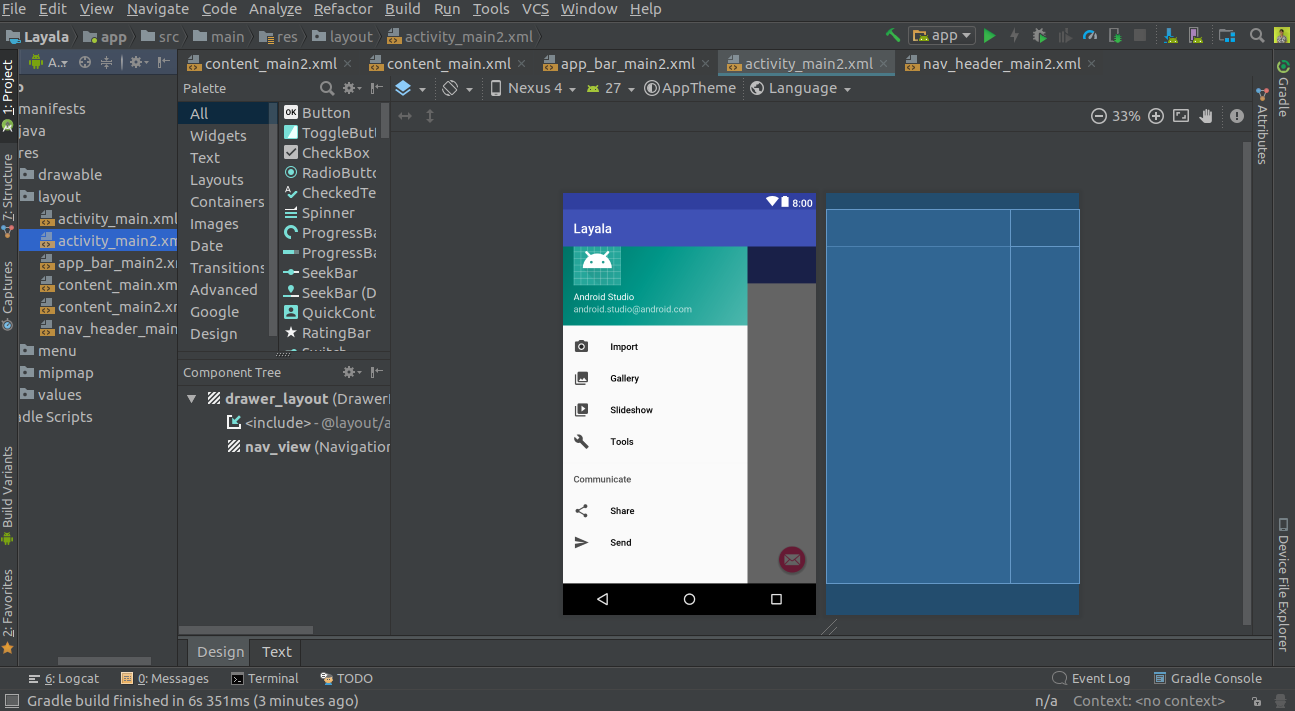
\includegraphics[width=0.7\textwidth]{img/interfaceEditing.png}
            \end{center}
        \caption{\label{fig:passaro}Edição de uma atividade do Android.}
        \begin{center}(FONTE: Imagem feita pelo autor)\end{center}
        \end{figure}

        Já o arquivo Java da atividade criada serve como uma controladora para a interface. Esse
        arquivo Java conterá uma classe que herda, indiretamente, da classe \textit{Activity}. O
        objetivo dessa classe é unicamente ser a controladora da ativdade que está sendo
        desenvolvida, ou seja, atualizar a interface e invocar métodos de outros objetos que tratem
        do modelo. Cada \textit{activity} tem sua própria controloradora e não deve gerenciar mais
        nenhuma outra interface, além da que foi designada. Outro ponto importante, é que alguns métodos
        herdados da classe \textit{Activity} tratam de eventos importantes como: atividade inicializada,
        resumida, suspensa, etc. Esses métodos são importantes, pois, por exemplo, caso o usuário
        venha a suspender o aplicativo que esteja executando para utilizar outro, o desenvolvedor
        pode utilizar o método \textit{onPause} para salvar dados importantes que o usuário tenha
        inserido até aquele momento.

        A aplicação desenvolvida também pode se comunicar com algum servidor ou ser uma aplicação
        que funciona apenas com dados locais. No primeiro caso, a aplicação funciona como um sistema
        web comum que segue o modelo de implementação cliente servidor. Sempre que for necessário
        utilizar dados do servidor para executar alguma ação, a aplicação fará uma requisição para
        o servidor através do protocolo HTTP para poder ter acesso as endpoints das APIS
        necessárias. Esse processo requer uma troca de dados estruturados. Ultimamente, muitas das
        API's que vem sendo implementadas tem utilizado apenas dados em formato JSON, mas já houve
        épocas em que o formato padrão era XML.

        \begin{figure}[htbp]
            \begin{center}
                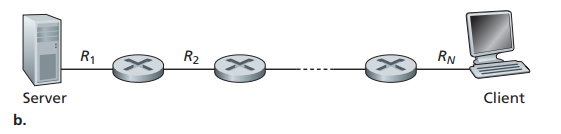
\includegraphics[width=0.7\textwidth]{img/clientServer.png}
            \end{center}
        \caption{\label{fig:passaro} Modelo Cliente servidor}
        \begin{center}(FONTE: KUROSE, J., KEITH, R. - Mobile, 2013)\end{center}
        \end{figure}

        Já no que se refere a dados locais, o Android utiliza, como ferramenta nativa, o banco de
        dados relacional \textit{SQLite}. Esse banco foi escolhido, visto que o propósito dele é
        unicamente ser um banco para sistemas embarcados e que utiliza apenas um único nodo
        computacional para fazer o acesso e atualização dos dados.

        Outro aspecto importante no desenvolvimento das aplicações para Android, é que o
        desenvolvedor pode testar o software sem precisar baixar em um aparelho
        físico. O Android Studio possui uma ferramenta nativa chamada Android Virtual
        Device (AVD), que permite emular os mais diversos aparelhos disponíveis no
        mercado, indepdente da marca ou segmento (i.e. tablets, celulares, TV's,
        \textit{Smartwatches}). Com essa plataforma, o desenvolvedor pode verificar como o seu
        software se comporta nos mais variados tamanhos de telas, bem como diferente
        tipos de configurações de hardware. Isso permite ao desenvolvedor garantir
        uma boa responsividade sem precisar pagar por novos aparelhos. Mesmo assim,
        é importante que quem esteja testando a aplicação faça os testes finais em
        dispositivos físicos para ver se a aplicação está se comportando da mesma
        forma como nos testes em ambiente de emulação, uma vez que os emuladores
        também estão abertos a falhas.

  \part{Trabalhos relacionados}

  \chapter{Trabalhos relacionados}
    Nesse capítulo são apresentados trabalhos relacionados que envolve tanto o desenvolvimento de frameworks,
    como ferramentas que ajudem na elaboração automática de testes automatizados. Os trabalhos aresentados
    ajudam, além de validar a exsitência desse trabalho, a reusar ideias já existentes e aplicá-las em um
    contexto específico, no caso aplicações atuais para a plataforma Android.

    \section{A busca de generalidade, flexibilidade e extensibilidade no processo de desenvolvimento de frameworks orientados a objetos}
      Nesse artigo (SILVA, Ricardo P. e, PRICE, R. T., 1998) é feito uma abordagem, resumida, dos principais conceitos envolvendo frameworks, a
      maioria deles já explicados no capítulo de Frameworks desse trabalho. Porém, um ponto importante
      discutido dentro desse artigo são os tópicos de padrões de projeto e metapadrões relacionados
      ao desenvolvimento de frameworks. Os padrões de projetos e metapadrões são contribuições
      importantíssimas , no que se refere a reuso de software. O trabalho comenta de um catálogo com
      23 padrões a serem seguidos pelos mais variados tipos de projetos e qual modelagem os projetos devem
      seguir. Já os metapadrões são mais independentes de domínio e visam a flexibilidade. Os templates são o
      principal exemplo disso dentro do artigo. Uma vez que os padrões de projetos são voltados a domínios
      específicos eles acabam sendo usados para o desenvolvimento de frameworks, porém os metapadrões não são
      completamente descartados, podendo ser utilizados quando for necessário dar alguma flexibilidade no
      algoritmo.

      O estudo comenta, de maneira superficial, o caminho que desenvolvedor deve seguir para desenvolver um
      framework, o qual seria: generalização, flexibilização, aplicação de metapadrões, aplicações de padrões
      de projeto e aplicações de boas práticas dentro da orientação a objetos.
      Na etapa de generalização, busca-se estudar as aplicações implementadas do domínio que será abordado
      e observar suas características compartilhadas, visando principalmente elementos comuns de domínio. A
      etapa de flexibilização seria identificar as pequenas variações de uma aplicação para outra. No caso do
      framework do artigo, foi generalizado o \textit{controller} responsável por processar a ação do usuário.
      Nos metapadrões, todos os jogos precisam ter tabuleiro e demais peças instanciadas. Para isso usou-se
      templates e hooks. Já para os padrões de projeto, utilizou-se os padrões observador e observável e
      \textit{abstract} e \textit{factory}. Também se utilizou o padrão \textit{decorator} no qual uma
      classe é responsável por realizar ações sobre o objeto que está sendo "decorado". Sobre as práticas
      de OO é comentado que a herança deve ser usada principalmente quando busca-se generalidade e concretizar classes abstratas.

      A principal contribuição do artigo para o trabalho são os conceitos de framework em si

    \section{An Object-Oriented Framework for Improving Software Reuse on Automated Testing of Mobile Phones}
      Frameworks capazes de auxiliar os desenvolvedores na elaboração de testes automatizados para aplicações
      mobile é um conceito que já foi aplicado no passado, como pode ser observado nesse artigo. Esse
      trabalho (SILVA, R. P., SANTOS, L. Et al., 2007) possui como principal foco o desenvolvimento de destes
      automatizados baseado em casos de uso, usando o reuso como principal forma de alcançar esse objetivo.
      No framework desenvolvido, ainda era necessário que o programador implementasse manualmente os testes.
      Porém, a grande vantagem do uso desse framework era que ele possuia grandes abstrações de hardware
      e se comunicava com o baixo nível através da API disponibilizada pela empresa que fabricava o
      telefone, no caso a Motorola, uma espécie de\textit{syscall}. A grande vantagem, era que o porte
      (i.e. executar os testes de um dispositivo em outro) podia ser feito sem necessidade de alterar o teste.

      Dos resultados obtidos do artigo, pode-se verificar que 10 modelos de celulares foram utilizados no
      estudo. A medida que os testes foram sendo portados para cada plataforma, o reuso aumentava
      consideravelmente, alcançando uma média de 84\% de reaproveitamento de testes. Fica nítido, através
      do estudo, também que o custo para automatizar testes é grande, visto que é o preço que se paga pelo
      reuso. Entretanto, ao portar testes de um modelo de celular para outro o esforço necessário é 1/4 do
      necessário se comparado ao esforço para escrever os testes, levando 1/3 do tempo. O artigo ainda
      aborda um estudo ao se utilizar 60 casos de teste passíveis de serem automatizados numa família de 15
      modelos de celulares. Neste cenário, inciou-se automatizando os testes mais simples. Enquanto certo
      teste não ficava pronto, ele era executado totalmente de forma manual. Além disso, baseado em quanto
      tempo levou-se para executar determinado teste manualmente, esse valor foi multiplicado pelo número de
      vezes que ele seria executado ao longo do projeto, a fim de melhor ajustar a estimativa. Neste estudo,
      o ganho de produtividade, no período de um ano, foi de três vezes, sendo que no terceiro mês de projeto,
      a automatização de testes já começou a se pagar.

      Nesse sentido, a principal contribuição do artigo para esse trabalho é, além de validar a importância
      do desenvolvimento de uma ferramenta similar para os dipositivos atuais, é utilizar o conceito de caso
      de uso para gerar testes automaticamente. A atual API do Android já é muito consolidada e e fornece
      abstrações o suficiente para que o programador não precise reescrever várias vezes a mesma aplicação
      para cada modelo de celular.

    \section{DroidMate: A Robust and Extensible Test Generator for Android}
      Esse artigo (JAMROZIK, K., ZELLER, A., 2016), é apresentado o DroidMate: uma ferramenta
      capaz de gerar testes baseado na interface de usuário combinado com testes
      exploratórios. O artigo inicia comentando da principal dificuldade de se escrever
      testes que é manter a base de testes sincronizada com a versão mais atual da aplicação.
      Isso acontece, visto que qualquer refatoração ou implementação de nova feature no sistema,
      ainda que seja mínima, necessita de uma revisão na base de testse. Dado esse cenário,
      é apresentado uma ferramenta capaz de monitorar o bytecode executado dentro da aplicação
      durante a utilização por um usuário. O framework implementado se propõe a criar
      um log utilziando como base as ações do usuário como cliques e texto
      digitado. Esse monitoramento é guardado em um arquivo do próprio framework. Após
      uma condição ser atendida, geralmente um \textit{timeout}, todo a ação monitorada
      é transformada em um teste para a aplicação.

      Para implementar esse teste gerado pela ferramenta, ele reusa o UiAutomator,
      uma ferramenta oficial do próprio Android voltada para o uso de testes de
      interface de usuário. O framework é capaz de gerar esse teste, já que durante
      o monitoramento de bytecode ele consegue ter acesso a \textit{stacktrace} de
      execução, chamada de funções e valores de parâmetros. Nesse sentido, ele
      combina os valores monitoardos junto com métodos disponibilizados no UiAutomator
      para criar os testes para o desenvolvedor.

      Sendo assim, a contribuição desse artigo para o esse trabalho se dá no fato de usar
      a interação do usuário com a aplicação, monitorada programaticamente, para gerar
      os testes de forma automática. Porém, diferente do DroidMate, o framework que
      será implementado buscar monitorar chamadas em mais alto nível, sem precisar fazer
      a verificação de cógido a nível de bytecode.

  \part{O framework}
    \chapter{Análise e desenvolvimento do framework}
      \section{Concepção}
        Dado os trabalhos apresentados no capítulo anterior, fica evidente que uma implementação
        para gerar automaticamente testes para dispositivos mobile é perfeitamente possível. O
        framework foi concebido sob a óptica de capturar as ações do usuário e gerar um teste
        a nível de interface de usuário. Porém, diferente do DroidMate, ao em vez de configurar
        um \textit{timeout}, será disponibilizado ao usuário configurar uma asserção para ser
        executada no final do teste, para verificar se houve sucesso ou não durante a ação
        do usuário.

        Além disso, o framework foi idealizado com a ideia de que o desenvolvedor não precise
        reescrever sua aplicação para se adequar a ferramenta. Nesse sentido, o framework
        foi desenvolvido com a ideia de que o desenvolvedor necessite apenas herdar classes
        do framework implementado e escreva algumas informações no arquivo de configuração.
        É importante deixar claro, que mesmo herdando as classes do framework, a aplicação
        desenvolvida não terá seu comportamento alterado de nenhuma maneira.

        Atualmente, a API do Android possui diversas chamadas de método que permitem detectar
        ações do usuário com a aplicação. Dentre todos os métodos disponíveis, destacam-se aqui
        os dois principais que permitiram a implementação do framework:
        \begin{description}
          \item[$\bullet$] \textit{public boolean dispatchTouchEvent(MotionEvent me)}
          \item[$\bullet$] \textit{public boolean dispatchKeyEvent(KeyEvent kEvent)}
        \end{description}

        Como os próprios nomes já sugerem, eles permitem detectar ações de clique do usuário
        e texto digitado, respectivamente. Esses métodos são invocados pelo Android toda
        vez que um evento de clique ou de digitação ocorre. Para o caso em que um clique
        é detectado, o objeto passado como parâmetro, \textit{MotionEvent}, permite coletar
        informações como posição em que o clique ocorreu (i.e. X e Y). Infelizmente essa classe
        não traz informações para detectar se o clique foi do tipo \textit{click and hold}, mas
        com uma lógica simples para verificar o tempo que levou para o clique iniciar e
        finalizar, é perfeitametne possível coletar esse tipo de informação. Uma lógica similar
        a essa é também utilizada para verificar se o clique foi do tipo \textit{scroll}. Para
        esse tipo de detecção, além de calcular o tempo de clique, é comparado a posição inicial
        com a posição final do clique.

        Para os eventos de digitação do usuário, o objeto passado como parâmetro no método, permite
        coletar qual foi a tecla digitada pelo usuário. Assim como o evento de clique, esse método é
        invocado pelo sistema operacional toda vez que um evento de digitação ocorre. É importante
        salientar que esses métodos são invocados duas vezes por evento: uma vez quando o evento é
        iniciado e outra quando o evento é finalizado. Dessa forma, a deteção de ações como
        \textit{scroll} e \textit{click and hold} é perfeitamente implementável do jeito como foi
        explicado anteriormente.

        Após o usuário finalizar as suas ações, o usuário deverá encerrar a apliação para indicar
        que suas ações terminaram. Após isso, o framework gera o teste com todos os atos feitos pelo usuário
        junto com a asserção definida previamente. Assim como o DroidMate, o framework utiliza
        a biblioteca UiAutomator para poder simular as ações do usuário. Escolheu-se essa biblioteca,
        pois além de ser a oficial da plataforma, ela é capaz de gerar cliques em posições X e Y.
        Para a função de asserção, o usuário deverá seguir as funções disponibilizadas no framework
        \textit{espresso}. Dessa forma, por utilizar esse framework internamente, a ferramenta
        desenvolvida foi batizada de \textit{capuccino}.

        Nesse sentido, o framework concebido acaba funcionando como uma espécie de proxy, em que as
        ações capturadas do usuário são guardadas em estrutura de dados da própria biblioteca, e o
        evento é então repassado oficialmente para aplicação, sem alterar nenhum valor ou comportamento
        original. Essas chamadas de método da API do Android estão disponíveis em toda \textit{Activity}
        e, como explicado no capítulo de desenvolvimento mobile, todo o desenvolvimento de uma aplicação
        Android se baseia em \textit{Activities}. Por isso, a principal função do \textit{capuccino} é
        reescrever esse métodos e solicitar ao desenvovledor que suas \textit{Activities} herdem daquela
        sobrescrita pelo framework.

      \section{Modelagem}
        A seguir é apresentada a modelagem em UML do \textit{capuccino}:

        \begin{figure}[htbp]
            \begin{center}
                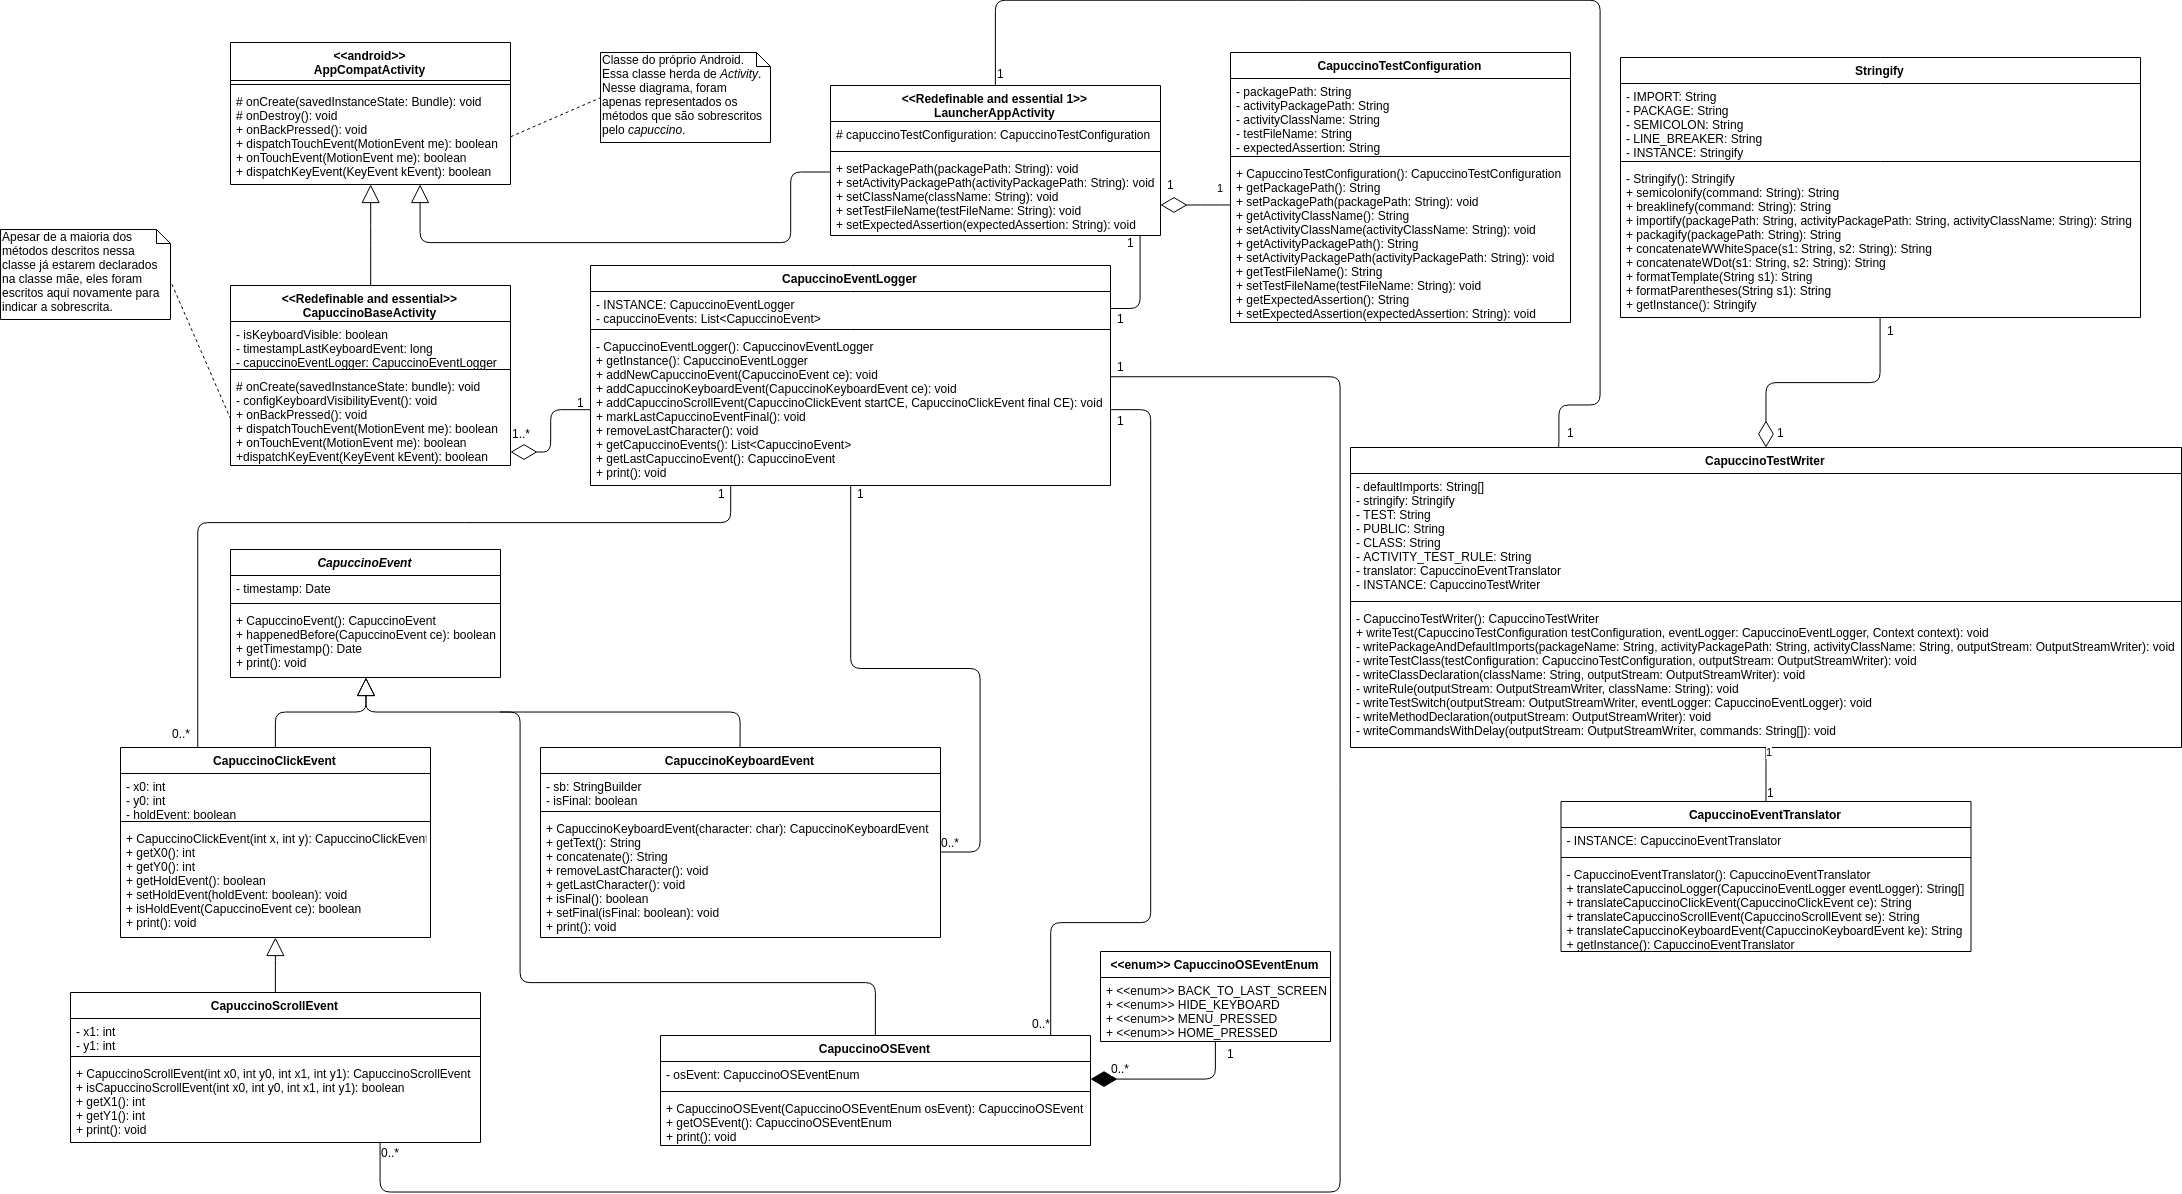
\includegraphics[width=1.0\textwidth]{img/capuccinoDiagram.png}
            \end{center}
            \caption{\label{fig:passaro} Diagrama de classes UML do framework Capuccino}
            \begin{center}(FONTE: Imagem feita pelo autor)\end{center}
        \end{figure}

        Como pode ser visualizado pelo diagrama, o \textit{capuccino} possui várias estrutura
        de dados (i.e. classes) para poder armazernar informações durante o processo de captura
        de ações do usuário. Mais detalhes sobre a implementação serão apresentados no próximo
        capítulo. Nesse capítulo busca-se destacar como que o desenvolvedor pode integrar sua aplicação
        com a ferramenta implementada. Para enteder isso, existem duas entidades chaves que são
        utilizadas para fazer essa integração. São elas:

        \begin{description}
          \item[$\bullet$] \textit{CapuccinoBasicActivity}
          \item[$\bullet$] \textit{LauncherAppActivity}
        \end{description}

        A classe \textit{LauncherAppActivity} é utilizada para inicar a aplicação do usuário. Além
        disso ela também serve para criar e configurar as informações que serão utilizadas para criar
        o teste automaticamente. Essa classe deve ser herdada pelo usuário e no arquivo \textit{AndroidManifest}
        de seu projeto deve configurar para que essa \textit{Activity} seja configurada o ponto
        de entrada da aplicação. Além de implementar essa herança, o usuário, dentro do método
        \textit{onCreate} deve usar os métodos \textit{setters} a fim de informar alguns dados
        para poder gerar o teste automaticamente de forma correta. Explicando breviamente cada um
        desses dados e sua respectiva importância:

        \begin{description}
          \item[$\bullet$] \textit{packagePath}: indica o \textit{package} da aplicação do usuário.
          \item[$\bullet$] \textit{activityPackagePath}: indica o \textit{package} onde a atividade a ser
                                                         ser testada se encontra. Esse caminho deve ser relativo
                                                         ao \textit{package} raiz.

          \item[$\bullet$] \textit{activityClassName}: nome da classe da atividade que será testada.
          \item[$\bullet$] \textit{testFileName}: nome do arquivo de teste que o desenvolvedor deseja que seja
                                                  gerado.

          \item[$\bullet$] \textit{expectedAssertion}:  asserção que o usuário quer que seja executada ao final do
                                                        do teste usando a sintaxe do \textit{espresso}.
        \end{description}

        Já a classe \textit{CapuccinoBasicActiviy} deve ser herdada por todas as atividades do usuário,
        ou pelo menos aquelas que serão testadas. Como dito anteriormente, o \textit{capuccino} funciona
        como uma proxy em que ele capta as ações do usuário e repassa para aplicação original. Quando
        o usuário herda suas atividades dessa classe é exatamente isso o que acontece. A
        \textit{CapuccinoBasicActiviy} está associada com ao \textit{CapuccinoEventLogger} que é responsável
        por manter os eventos ordenados por horário em que ocorreu em uma lista.


      \section{Implementação}
      \section{Limitações da ferramenta}


  \part{Resultados obtidos}
    TODO

  % \chapter{Testando o Framework}

  % \part{Resultados e trabalhos futuros}

  % \chapter{Resultados obtidos}

  % \chapter{Sugestões de trabalhos futuros}

  % \chapter{Conclusão}



  % ---
  % Finaliza a parte no bookmark do PDF, para que se inicie o bookmark na raiz
  % ---
  % \bookmarksetup{startatroot}%
  % ---

  % ---
  % Conclusão
  % ---

  % \lipsum[31-33]

  % ----------------------------------------------------------
  % ELEMENTOS PÓS-TEXTUAIS
  % ----------------------------------------------------------
  \postextual


  % ----------------------------------------------------------
  % Referências bibliográficas
  % ----------------------------------------------------------
  \bibliography{abntex2-modelo-references}
  \chapter*{Referências}
  \noindent
  WAZLAWICK, R. S. \textit{Engenharia de Software para Sistemas de Informações: Conceitos e práticas que fazem sentido}. Florianópolis [s.n.], 2012.

  \noindent
  DIJKSTRA, E. W. \textit{The Humble Programmer}. [S.I], 1971. Disponível em:
  \url{https://www.cs.utexas.edu/~EWD/transcriptions/EWD03xx/EWD340.html}.
  Acesso em 2 de Setembro de 2017.

  \noindent
  JEREMIAH, J. \textit{Is agile the new norm?}. [S.I.:s.n.], 2017 Disponível em:
  \url{https://techbeacon.com/survey-agile-new-norm}. Acesso em 2 de Setembro de 2017.

  \noindent
  KELLY, A. \textit{Programmers Without TDD Will be Unemployable by 2022}. [S.I.:s.n.],
  2014 Disponível em: \url{https://dzone.com/articles/programmers-without-tdd-will}. Acesso em 22 de Abril de 2018.

  \noindent
  ERIKSSON, U. \textit{How much time should you spend on testing?}. [S.I.:s.n.], 2014 Disponível em:
  \url{https://goo.gl/bTfQsa}. Acesso em 2 de Setembro de 2017.

  \noindent
  SILVA, Ricardo P. e, PRICE, R. T. \textit{A busca de generalidade, flexibilidade e extensibilidade no processo de desenvolvimento de frameworks orientados a objetos}. [S.I.:s.n.], 1998 Disponível em: \url{https://www.inf.ufsc.br/~ricardo.silva/publications/Ideas98.PDF}. Acesso em 4 de Março de 2018.

  \noindent
  \textit{Software design pattern}. In: Wikipédia, a enciclopédia livre. Flórida: Wikimedia Foundation,
  2018. Disponível em:
  \url{https://en.wikipedia.org/w/index.php?title=Software_design_pattern&oldid=834346932}. Accesso
  em 19 de Abril 2018.

  \noindent
  JOHNSON, R. E. \textit{Design Patterns: Abstraction and Reuse of Object-Oriented Design}. [S.I.:s.n.], 1993 Disponível em: \url{https://link-springer-com.ez46.periodicos.capes.gov.br/chapter/10.1007%2F3-540-47910-4_21}. Acesso em 26 de Março de 2018.

  \noindent
  KENT, B., ANDRES, C. \textit{Extreme Programming Explained}. [S.I.:s.n.], 2004.

  \noindent
  ERIKSSON, U. \textit{3 Reasons Why It's Important to Refactor Tests}. [S.I.:s.n.], 2016 Disponível em:
  \url{https://qualitycoding.org/why-refactor-tests/#comments}. Acesso em 4 de Maio de 2018.

  \noindent
  FOWLER, M. \textit{Making Stubs}. [S.I.:s.n.], 2003 Disponível em:
  \url{https://martinfowler.com/bliki/MakingStubs.html}. Acesso em 4 de Maio de 2018.

  \noindent
  FOWLER, M. \textit{Test Pyramid}. [S.I.:s.n.], 2012 Disponível em:
  \url{https://martinfowler.com/bliki/TestPyramid.html}. Acesso em 4 de Maio de 2018.

  \noindent
  BAGMAR, A. \textit{Behavior Driven Testing (BDT) in Agile}. [S.I.:s.n.], 2012 Disponível em:
  \url{https://www.slideshare.net/abagmar/anand-bagmar-behavior-driven-testing-bdt-in-agile}. Acesso em 2 de Junho de 2018.

  \noindent
  KHAN, M. E., KHAN, F. \textit{A Comparative Study of White Box, Black Box and Grey Box Testing Techniques}. [S.I.:s.n.], 2012 Disponível em: \url{http://citeseerx.ist.psu.edu/viewdoc/download?doi=10.1.1.261.1758&rep=rep1&type=pdf}. Acesso em 2 de Junho de 2018.

  \noindent
  \textit{Number of available applications in the Google Play Store from December 2009 to March 2018}.
  [S.I.:s.n.], 2018 Disponível em: \url{https://www.statista.com/statistics/266210/number-of-available-applications-in-the -google-play-store/}. Acesso em 2 de Junho de 2018.

  \noindent
  \textit{MOBILE (ANDROID) HARDWARE STATS 2017-03}. [S.I.:s.n.], 2018 Disponível em: \url{https://web.archive.org/web/20171113032047/https://hwstats.unity3d.com/mobile/cpu-android.html}. Acesso em 2 de Junho de 2018.

  \noindent
  HALPERN, M., ZHU, Y., REDDI, V. J. \textit{Mobile CPU’s Rise to Power: Quantifying the Impact of Generational Mobile CPU Design Trends on Performance, Energy, and User Satisfaction}.
  [S.I.:s.n.], 2016 Disponível em: \url{http://matthewhalpern.com/publications/mobile-cpus-hpca-2016.pdf}. Acesso em 1 de Junho de 2018.

  \noindent
  \textit{Android (operating system)}. In: Wikipédia, a enciclopédia livre. Flórida: Wikimedia Foundation,
  2018. Disponível em:
  \url{https://en.wikipedia.org/wiki/Android_(operating_system)}. Accesso
  em 2 de Junho 2018.

  \noindent
  \textit{Smartphone OS}. [S.I.:s.n.], 2018 Disponível em: \url{https://www.idc.com/promo/smartphone-market-share/os}.
  Acesso em 2 de Junho de 2018.

  \noindent
  KUROSE, J., KEITH, R.\textit{Computer Networking A Top-Down Approach}. [S.I.:s.n.], 2013 Disponível em: \url{http://www.bau.edu.jo/UserPortal/UserProfile/PostsAttach/10617_1870_1.pdf}. Acesso em 14 de Junho de 2018.

  \noindent
  KAWAKAMI, L., KNABBEN A., RECHIA, D., BASTOS, D., PEREIRA, O., SILVA, R. P., SANTOS, L. \textit{An Object-Oriented Framework for Improving Software Reuse on Automated Testing of Mobile Phones}. IFIP 19th TESTCOM - 7th FATES. Tallinn, 2007

  \noindent
  SILVA, Ricardo P. e, PRICE, R. T. \textit{A busca de generalidade, flexibilidade e extensibilidade no processo de desenvolvimento de frameworks orientados a objetos}.
  In: Proceedings of Workshop Iberoamericano de Engenharia de Requisitos e Ambientes de Software (IDEAS'98). Torres: apr. 1998. v.2, p.298-309.

  \noindent
  JAMROZIK, K., ZELLER, A.  \textit{DroidMate: A Robust and Extensible Test Generator
  for Android}. ACM International Conference on Mobile Software Engineering and Systems (MOBILESoft), 2016 Disponível em: \url{http://www.boxmate.org/files/DroidMate_MOBILESoft_2016.pdf}. Acesso em 1 de Junho de 2019.

  \noindent


  % ----------------------------------------------------------
  % Glossário
  % ----------------------------------------------------------
  %
  % Consulte o manual da classe abntex2 para orientações sobre o glossário.
  %
  %\glossary

  % ----------------------------------------------------------
  % Apêndices
  % ----------------------------------------------------------

  % ---
  % Inicia os apêndices
  % ---
  % \begin{apendicesenv}

  % Imprime uma página indicando o início dos apêndices
  % \partapendices

  % ----------------------------------------------------------
  % \chapter{Quisque libero justo}
  % ----------------------------------------------------------

  % \lipsum[50]

  % ----------------------------------------------------------
  % \chapter{Nullam elementum urna vel imperdiet sodales elit ipsum pharetra ligula
  % ac pretium ante justo a nulla curabitur tristique arcu eu metus}
  % ----------------------------------------------------------
  % \lipsum[55-57]

  % \end{apendicesenv}
  % ---


  % ----------------------------------------------------------
  % Anexos
  % ----------------------------------------------------------

  % ---
  % Inicia os anexos
  % ---
  % \begin{anexosenv}

  % Imprime uma página indicando o início dos anexos
  % \partanexos

  % ---
  % \chapter{Morbi ultrices rutrum lorem.}
  % ---
  % \lipsum[30]

  % ---
  % \chapter{Cras non urna sed feugiat cum sociis natoque penatibus et magnis dis
  % parturient montes nascetur ridiculus mus}
  % ---

  % \lipsum[31]

  % ---
  % \chapter{Fusce facilisis lacinia dui}
  % ---

  % \lipsum[32]

  % \end{anexosenv}

  %---------------------------------------------------------------------
  % INDICE REMISSIVO
  %---------------------------------------------------------------------

  \printindex

  \end{document}
